\documentclass[11pt,letterpaper]{article}
\usepackage[margin=1in]{geometry}
\usepackage[T1]{fontenc}
\usepackage[utf8]{inputenc}
\usepackage{lmodern}
\usepackage{amsmath,amssymb}
\usepackage{array,longtable}
\usepackage{xcolor}
\usepackage{listings}
\usepackage{seqsplit}
\usepackage{graphicx}
\usepackage{float}
\usepackage{microtype}
\usepackage[hidelinks]{hyperref}
\setlength{\parindent}{0pt}
\setlength{\parskip}{6pt}
\setlength{\emergencystretch}{3em}
\lstset{basicstyle=\ttfamily\scriptsize,breaklines=true,
  breakatwhitespace=false,columns=fullflexible,keepspaces=true,
  showstringspaces=false,frame=single,rulecolor=\color{gray!40},
  commentstyle=\color{black!60},tabsize=4}
\title{Programmable Birdsong Synthesizer\\\large ECE 4760: Laboratory 1}
\author{Kaelem Bent (kab472), Ruth Taddesse (ryt5)}
\date{Thursday, September 24th, 2026}
\begin{document}
\maketitle

\section*{1. Introduction}

We built a birdsong synthesizer with a Raspberry Pi Pico 2, a slide potentiometer, a keypad, and an SPI digital-to-analog converter (DAC). Moving the potentiometer changes the tone's frequency over a nominal 0--10 kHz range. We can save a different sound to each key from 1 to 9 and play it back faster. The keypad also lets us mute the tone and put saved sounds together into a sequence. While entering a sequence, each sound plays as we press its key, much like a soundboard.

The audio runs in a timer interrupt using direct digital synthesis (DDS). Separate protothreads handle the keypad, potentiometer, recording, playback, and volume changes. We only save the frequency as it changes, so we do not need to store every audio sample. Playing those saved values back ten times faster makes the frequency sweep happen faster while keeping the same pitch range.

We followed the ECE 4760 requirements for \href{https://vanhunteradams.com/Pico/Birds/Birdsong.html}{Synthesizing Birdsong with the RP2350}. We started with the DAC and ADC examples, then added recording and composition. We did not implement the extra volume-switch feature listed for ECE 5730.

\section*{2. Design and Testing Methods}

\subsection*{2.1 Incremental development and milestone mapping}

We kept separate files as we added features. The table below shows which file goes with each checkpoint and what we can show from the code or lab photos. The files explain how the project developed, but they do not replace measurements from the hardware.

\begingroup\small
\setlength{\tabcolsep}{5pt}
\begin{longtable}{|>{\raggedright\arraybackslash}p{0.295\linewidth}|>{\raggedright\arraybackslash}p{0.295\linewidth}|>{\raggedright\arraybackslash}p{0.295\linewidth}|}
\hline
\textbf{Checkpoint} & \textbf{Repository evidence} & \textbf{Implementation / available evidence} \\ \hline
\endhead
Preparation: build course examples & Pico SDK import and CMake project & Current CMake configuration selects the final application \\ \hline
Week 1: fixed tone and DAC output & \texttt{dactest.c}: 800 Hz DDS command, channel A & Supplied scope photograph displays 800.000 Hz \\ \hline
Week 1: change DAC channel & \texttt{dactest\_other\_channel.c}: channel B control word & Channel-B control word appears in the separate test program \\ \hline
Week 1: external boot button & Build links \texttt{pico\_bootsel\_via\_double\_reset} & Software support is present; external button wiring is not established by the source \\ \hline
Week 1: potentiometer and ADC & \texttt{ADC\_with\_DDS.c}: ADC channel 0 mapped to 0--10,000 Hz & Nominal range is defined by the ADC-to-frequency mapping \\ \hline
Week 2: keypad integration and mute & \texttt{ADC\_DDS\_keypad\_mute.c}: four-state debounce and amplitude ramp & Debounce logic and bounded amplitude control are implemented \\ \hline
Week 2: nine recordings and normal-speed playback & \texttt{ADC\_DDS\_keypad\_record.c}: frequency buffers and 10 ms playback & Separate frequency buffers store sounds for keys 1--9 \\ \hline
Week 2: interrupt timing & GPIO 2 surrounds synthesis ISR & Supplied timing trace: 1.63 \ensuremath{\mu}s pulse and 50 kHz readout \\ \hline
Week 3: live tone at boot and return via 0 & \texttt{ADC\_DDS\_keypad\_speedup.c}: initial tone enabled; mode cancellation on 0 & Initial tone enabled; key 0 restores live potentiometer control \\ \hline
Week 3: accelerated playback & Final file: 10 ms record, 1 ms playback & Nominal 10:1 ratio from the programmed update intervals \\ \hline
Week 3: composition and sound previews & Final file: nine-entry sequence; indirect lookup of stored sound & Stored key sequence selects recorded sounds; previews are enabled \\ \hline
Week 3: demonstration without restart & Final state transitions support repeated operation & Supplied screenshot documents Northern Cardinal identification \\ \hline
\end{longtable}
\endgroup

The older files show the earlier stages of the project. Our current CMake file builds only \texttt{ADC\_DDS\_keypad\_speedup.c}; the older files may differ from the versions used during checkout.

\subsection*{2.2 Hardware approach}

We set SPI0 to send 16-bit words at a requested clock rate of 20 MHz, with clock polarity and phase both set to zero. Each word contains the channel-A settings and a 12-bit output value. The command enables the channel at a gain of one. The lab specifies an MCP4822 DAC, although the part number is not readable in our breadboard photos.

The potentiometer wiper connects to GPIO 26, or ADC input 0. The two ends need to connect to the supply and ground so the wiper stays within the ADC's input range. We use GPIO 9--12 for the keypad rows and GPIO 13--15 for the columns, with pull-ups on the column inputs. To scan a key, the code drives one row low, waits 1 microsecond, and reads the columns. It then compares the input with a lookup table to find the key.

The block diagram shows how signals move through the program, and the pin table lists the GPIO assignments. These do not show every breadboard connection. Details such as the DAC latch, power wiring, boot button, and audio-jack connections would need a separate wiring diagram.

The first photo shows our early DAC setup with the audio socket and scope probes connected. The second shows the later setup with the potentiometer and keypad added. Some wires are hidden, so the photos alone are not enough to trace every connection.

\begin{figure}[H]
\centering
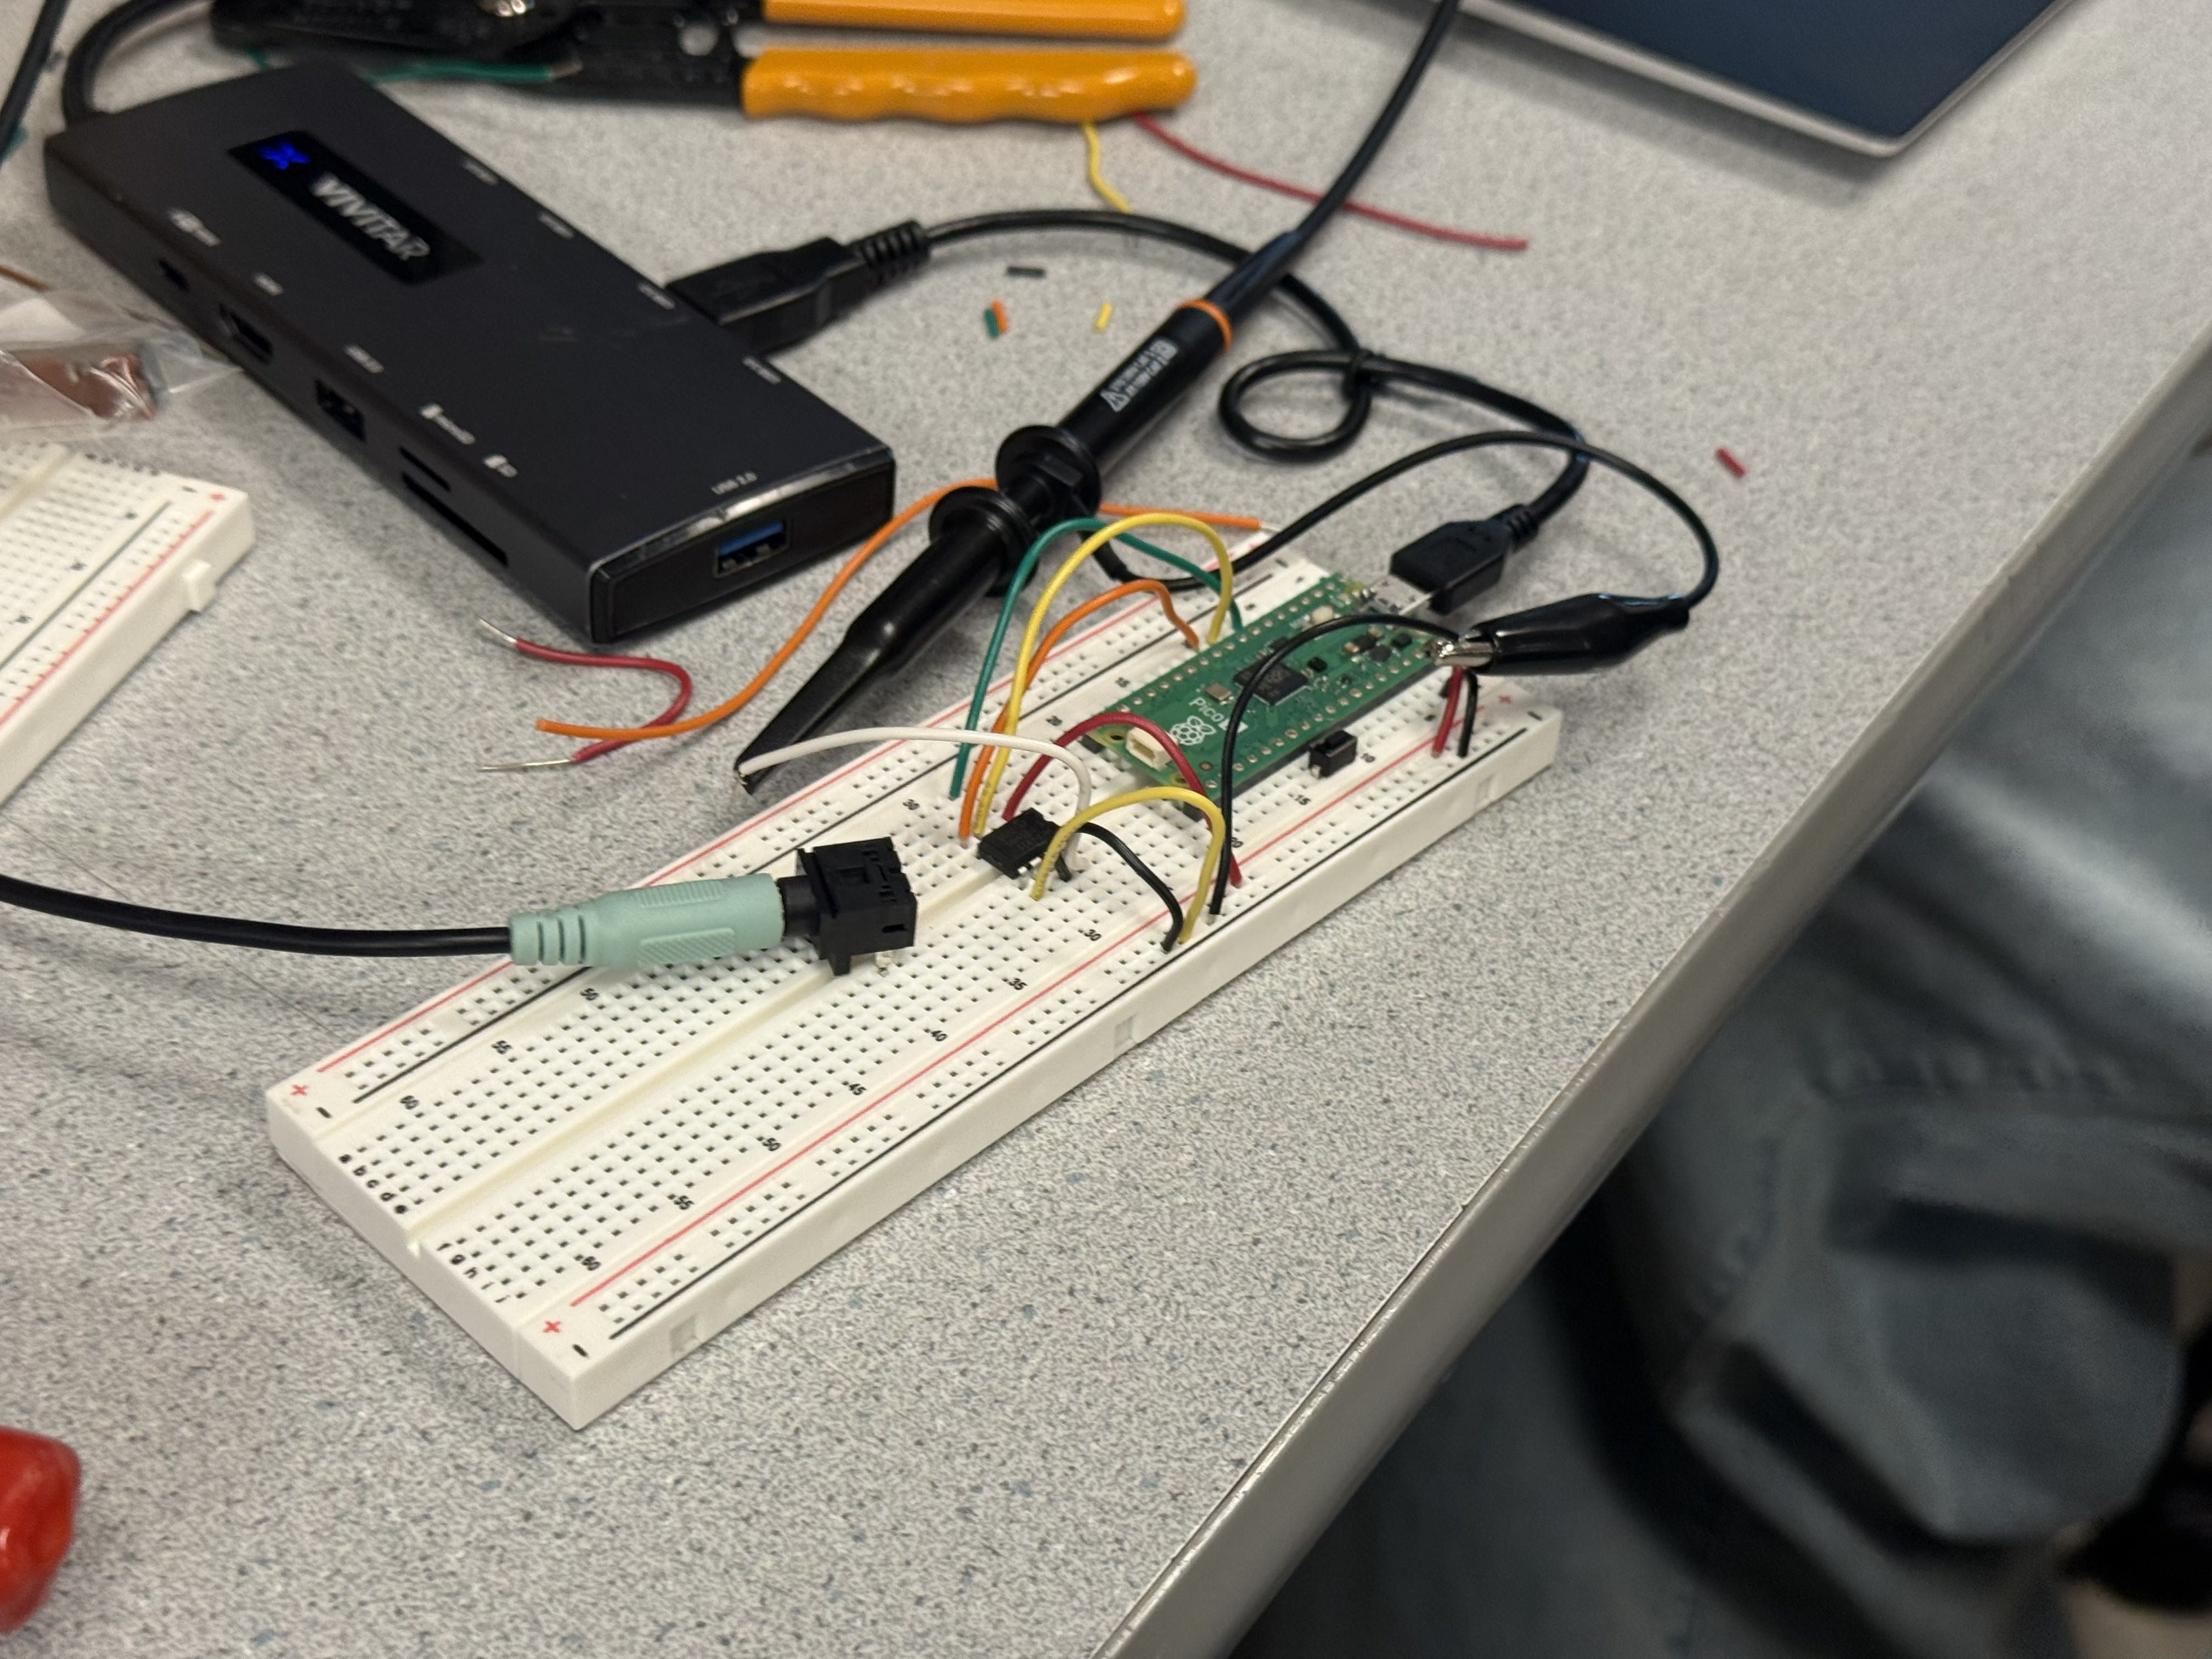
\includegraphics[width=\linewidth,height=0.65\textheight,keepaspectratio]{figures/dac_breadboard.jpg}
\caption{Initial DAC and audio-output breadboard setup, including the controller, audio socket, USB connection, and oscilloscope probes. Photograph: IMG\_7768.}
\end{figure}

\begin{figure}[H]
\centering
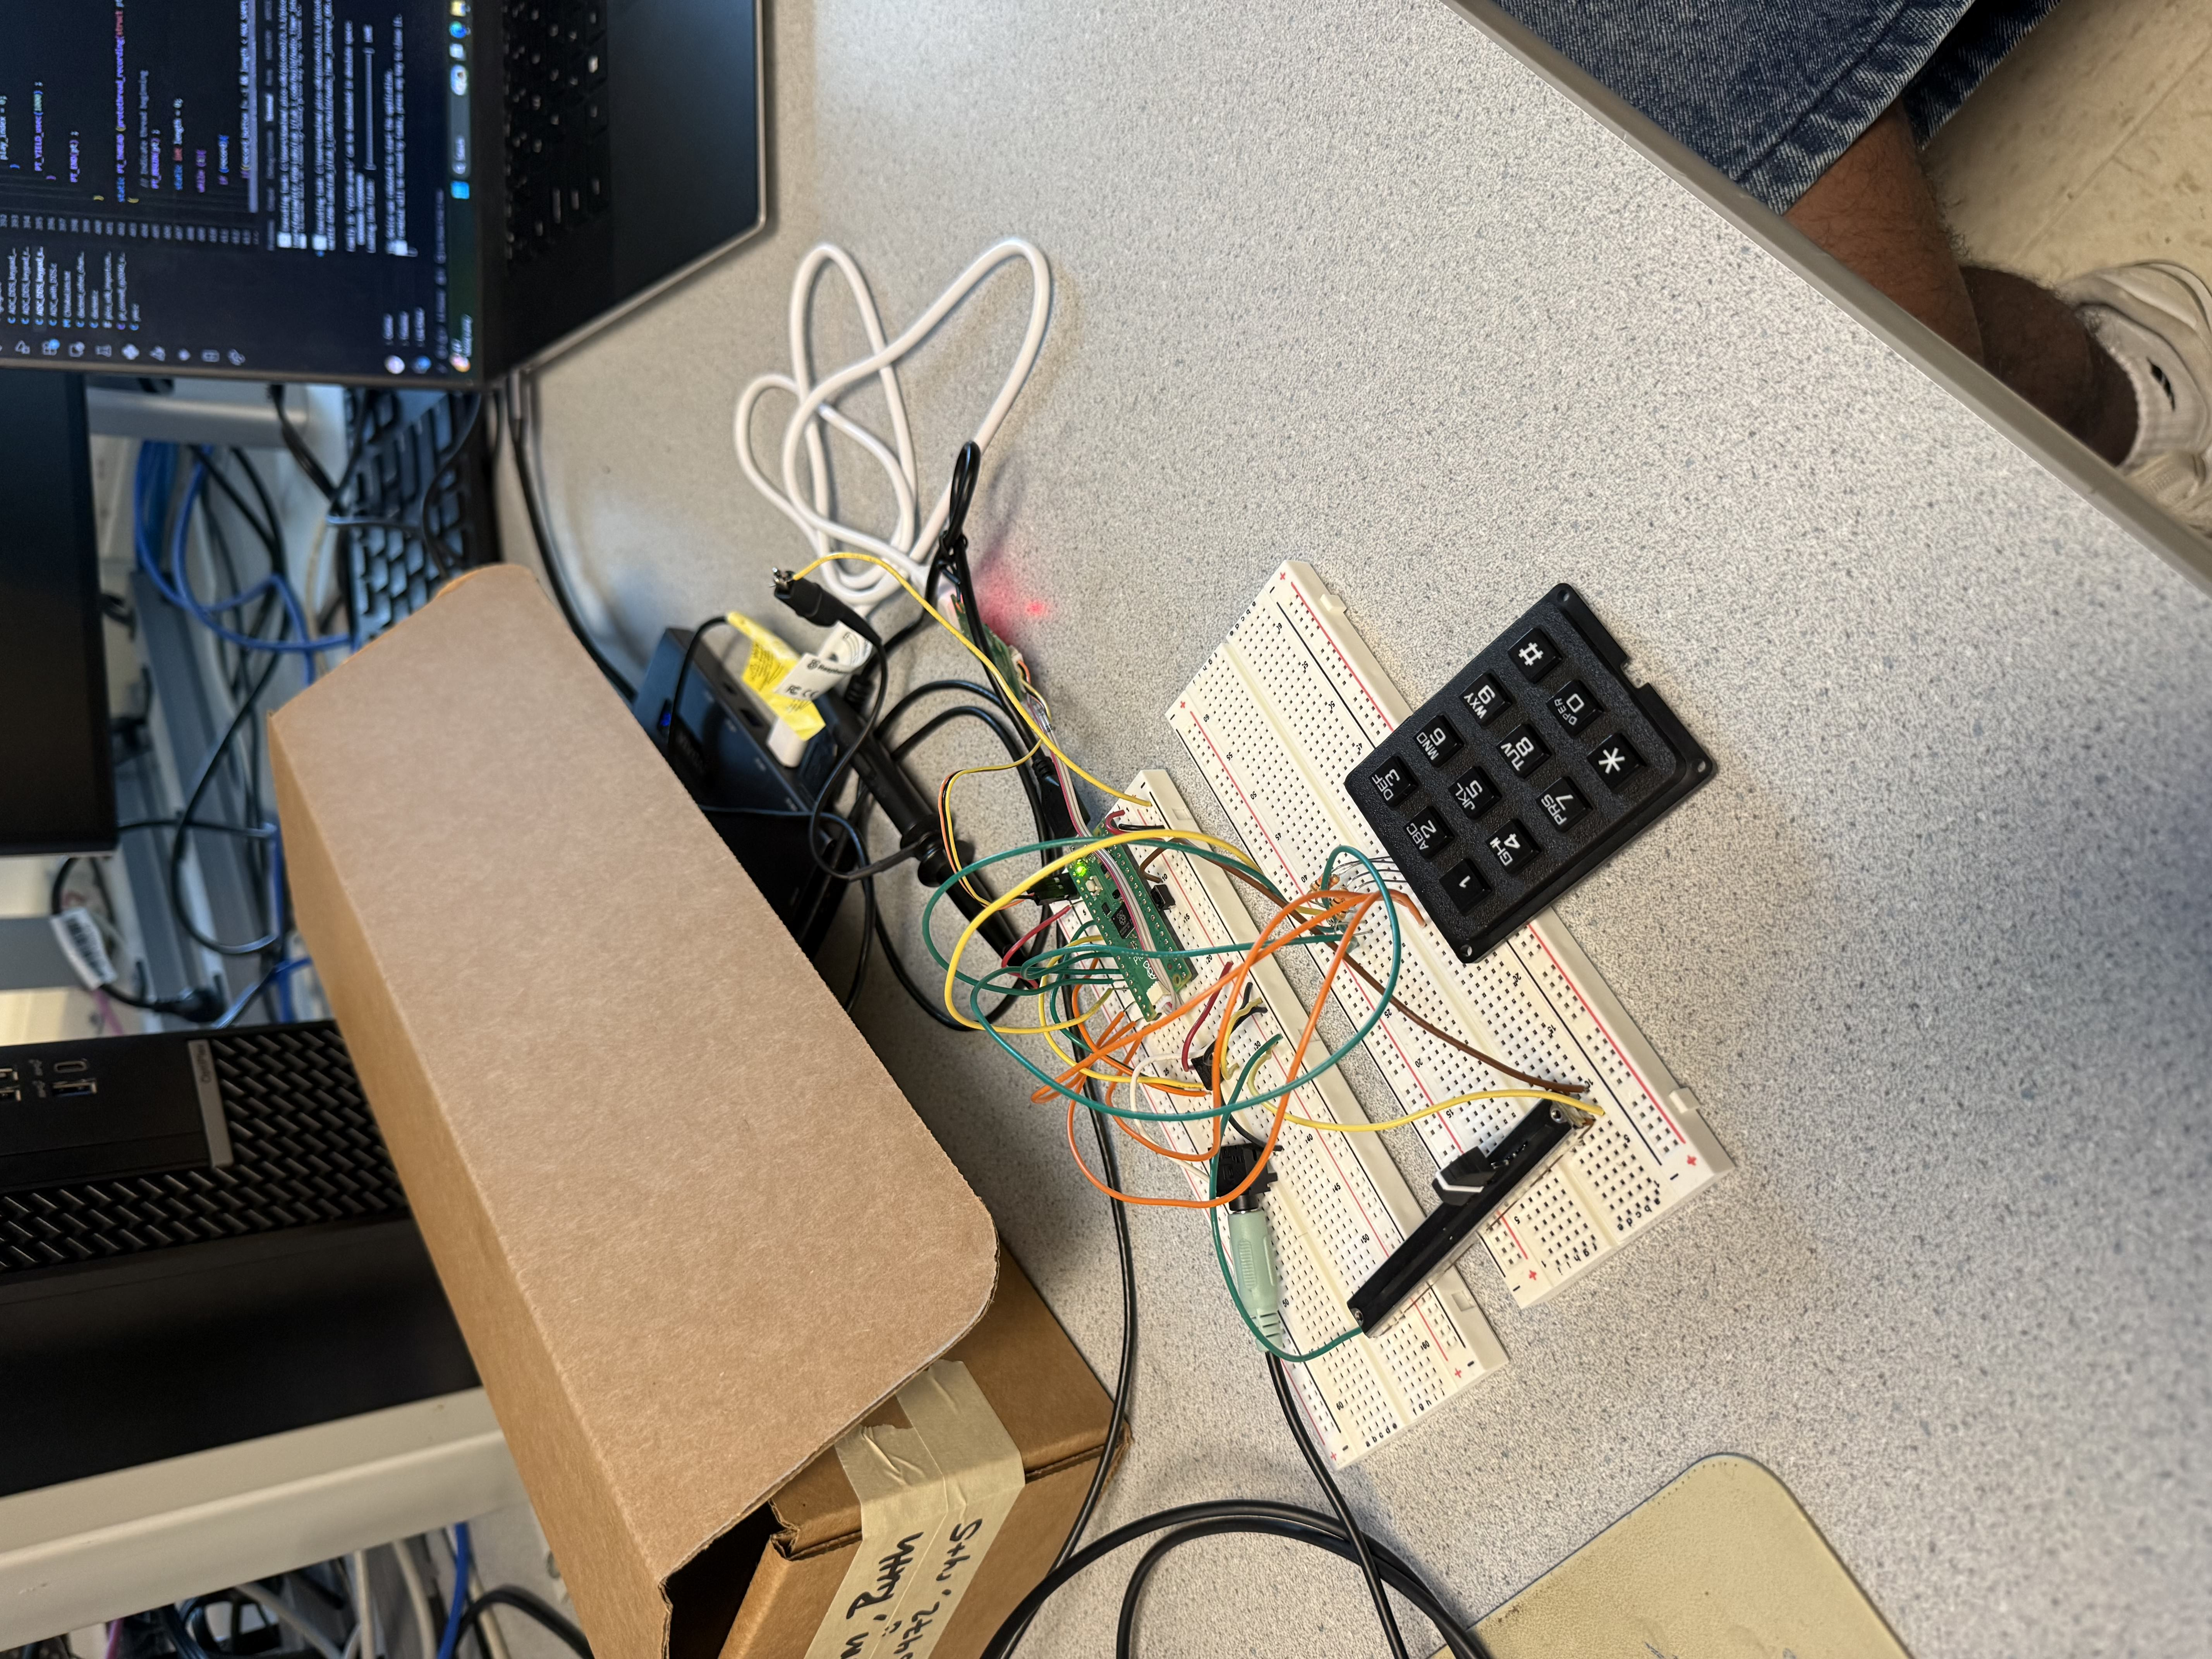
\includegraphics[angle=-90,width=\linewidth,height=0.65\textheight,keepaspectratio]{figures/keypad_potentiometer_setup.jpg}
\caption{Integrated synthesizer setup with the slide potentiometer, matrix keypad, controller, and audio-output wiring. Photograph: IMG\_7908.}
\end{figure}

\subsection*{2.3 DDS and amplitude control}

We convert the ADC reading a into a frequency using integer arithmetic:

\texttt{f\_command = floor(a \ensuremath{\times} 10000 / 4095)} Hz.

That frequency gives us the phase increment:

\texttt{\ensuremath{\Delta} = floor(f\_command \ensuremath{\times} 2\textasciicircum{}32 / 50000)}.

Each interrupt adds \ensuremath{\Delta} to a 32-bit unsigned phase accumulator. When it overflows, it wraps back around. We use the top eight bits to choose one of the 256 sine-table entries. The table is filled with \texttt{2047 \ensuremath{\times} sin(2\ensuremath{\pi}i/256)}, using 6.283 for 2\ensuremath{\pi}. Before sending a sample to the DAC, we scale it by the amplitude and add the midpoint offset:

\texttt{DAC\_code = 2048 + trunc(sine\_table[phase >> 24] \ensuremath{\times} amplitude / 2047)}.

At full amplitude, the output codes stay between 1 and 4095. When muted, the DAC stays at code 2048. This removes the changing part of the signal instead of setting the output to zero volts. The phase accumulator still runs while the sound is muted.

We keep amplitude between 0 and 2047. The amplitude thread changes it by 103 each time it runs, then yields for 50 microseconds. It takes 20 updates to go from silent to full volume, or roughly 1 ms plus scheduling delays. An old comment still says the updates are 1 ms apart, which was true in the earlier mute version. The final code uses the shorter delay. The ramp happens when playback starts or stops, but it does not restart for each sound in a composition.

\subsection*{2.4 Recording, playback, and concurrency}

All five protothreads run on the default core scheduler. We included some multicore, DMA, and PIO headers from the examples, but the final program does not use those features.

\begingroup\small
\setlength{\tabcolsep}{5pt}
\begin{longtable}{|>{\raggedright\arraybackslash}p{0.295\linewidth}|>{\raggedright\arraybackslash}p{0.295\linewidth}|>{\raggedright\arraybackslash}p{0.295\linewidth}|}
\hline
\textbf{Routine} & \textbf{Role} & \textbf{Requested yield} \\ \hline
\endhead
\texttt{protothread\_toggle25} & Read ADC, print commanded frequency, update live-tone increment when playback is inactive & 10 ms \\ \hline
\texttt{protothread\_core\_0} & Scan keypad, debounce, dispatch mode actions & 30 ms \\ \hline
\texttt{protothread\_amplitude} & Move amplitude toward its enabled/muted target & 50 \ensuremath{\mu}s \\ \hline
\texttt{protothread\_playback} & Select successive frequencies from an individual sound or composition & 1 ms \\ \hline
\texttt{protothread\_recording} & Append frequency values while recording & 10 ms \\ \hline
\texttt{alarm\_irq} & Advance DDS and transfer DAC sample & Nominal 20 \ensuremath{\mu}s alarm interval \\ \hline
\end{longtable}
\endgroup

We store sounds in \texttt{uint16\_t sounds[9][1000]} and track the number of saved values for each key. Key k uses row k\ensuremath{-}1. The array takes 18,000 bytes and holds about ten seconds per key at 100 samples per second. Recording saves one frequency about every 10 ms; playback reads one about every 1 ms. This makes a recording play in roughly one-tenth the time. We leave the DAC sample rate and the saved frequency values unchanged.

While idle, the recording thread resets its write index to zero. During recording, it writes the next frequency and updates that sound's length. If the array fills up, it stops adding samples until the key is released. All sounds are stored in RAM, so they disappear when the board resets or loses power. A composition only saves key numbers. If we later replace a sound, a saved composition using that key will play the new version.

The ADC thread stops updating \texttt{phase\_incr\_main} whenever a sound or composition is playing. Otherwise, the potentiometer would overwrite the saved frequency. Changing modes stops the other playback and resets the playback positions. Key 0 takes us back to the potentiometer, or toggles mute if we are already in tone-generator mode. In compose mode, pressing a digit adds it to the sequence and plays its sound if one is saved. Pressing hash again stops that preview and starts the whole sequence from the beginning.

\subsection*{2.5 Testing methods}

We checked the output waveform, ISR timing, and whether the sound was recognizable as birdsong. The first test program commands an 800 Hz tone. Our scope photo shows a sine wave with an 800.000 Hz readout, matching that setting. We also have a separate program that selects DAC channel B, but we do not have a separate measurement photo for that output.

To check how long the ISR takes, we set GPIO 2 high when it starts and low just before it returns. The time between those edges shows how long the code between the two GPIO writes takes. Our scope capture shows 1.63 microseconds and a 50 kHz frequency readout. This is one captured pulse, so we cannot call it the longest possible ISR time.

For the keypad, the main checks are that a held key causes only one press action, that holding a digit records its frequency changes, and that pressing it again plays the saved sound. Composition adds another check: the saved sounds should play in the entered order, with previews still working while we enter the sequence. These behaviors can be traced through the code, but we did not record a numerical failure rate.

We played our synthesized birdsong to Merlin Sound ID during the final demonstration. It identified a Northern Cardinal. The screenshot includes the identification and Merlin's live spectrogram. For playback speed, we report the nominal tenfold increase from the 10 ms recording and 1 ms playback delays. We do not have a separate measurement of the actual duration ratio.

\subsection*{2.6 Use of AI}

We used an AI coding assistant to help explain DDS, review our debounce logic, and check the recording and composition code. We asked about amplitude control, missing switch breaks, array sizes, and the difference between storing a frequency and storing a phase increment. Later questions focused on playback speed, sequence indexing, and resetting modes. Most of the time, we asked for suggestions without file changes and made the edits ourselves.

In one earlier version, the assistant directly shortened the fade, moved the toggle to a release transition, added thread registrations, and removed an undefined LED reference. We did not keep every suggestion in later versions. For example, the final code still handles most controls on confirmed press. Other suggestions that remain include fixed-size frequency arrays, amplitude limits, looking up sounds through the composition sequence, and using key 0 to return to the live tone.

We reviewed the suggestions against our code rather than treating them as test results. The scope readings and Merlin result come from our lab images. Appendix B summarizes the code-development conversation and explains what is missing from the full prompt log. Exact counts of suggested and accepted changes still need the complete conversation.

\section*{3. Documentation}

\subsection*{3.1 Logical wiring and signal flow}

\begin{figure}[H]
\centering
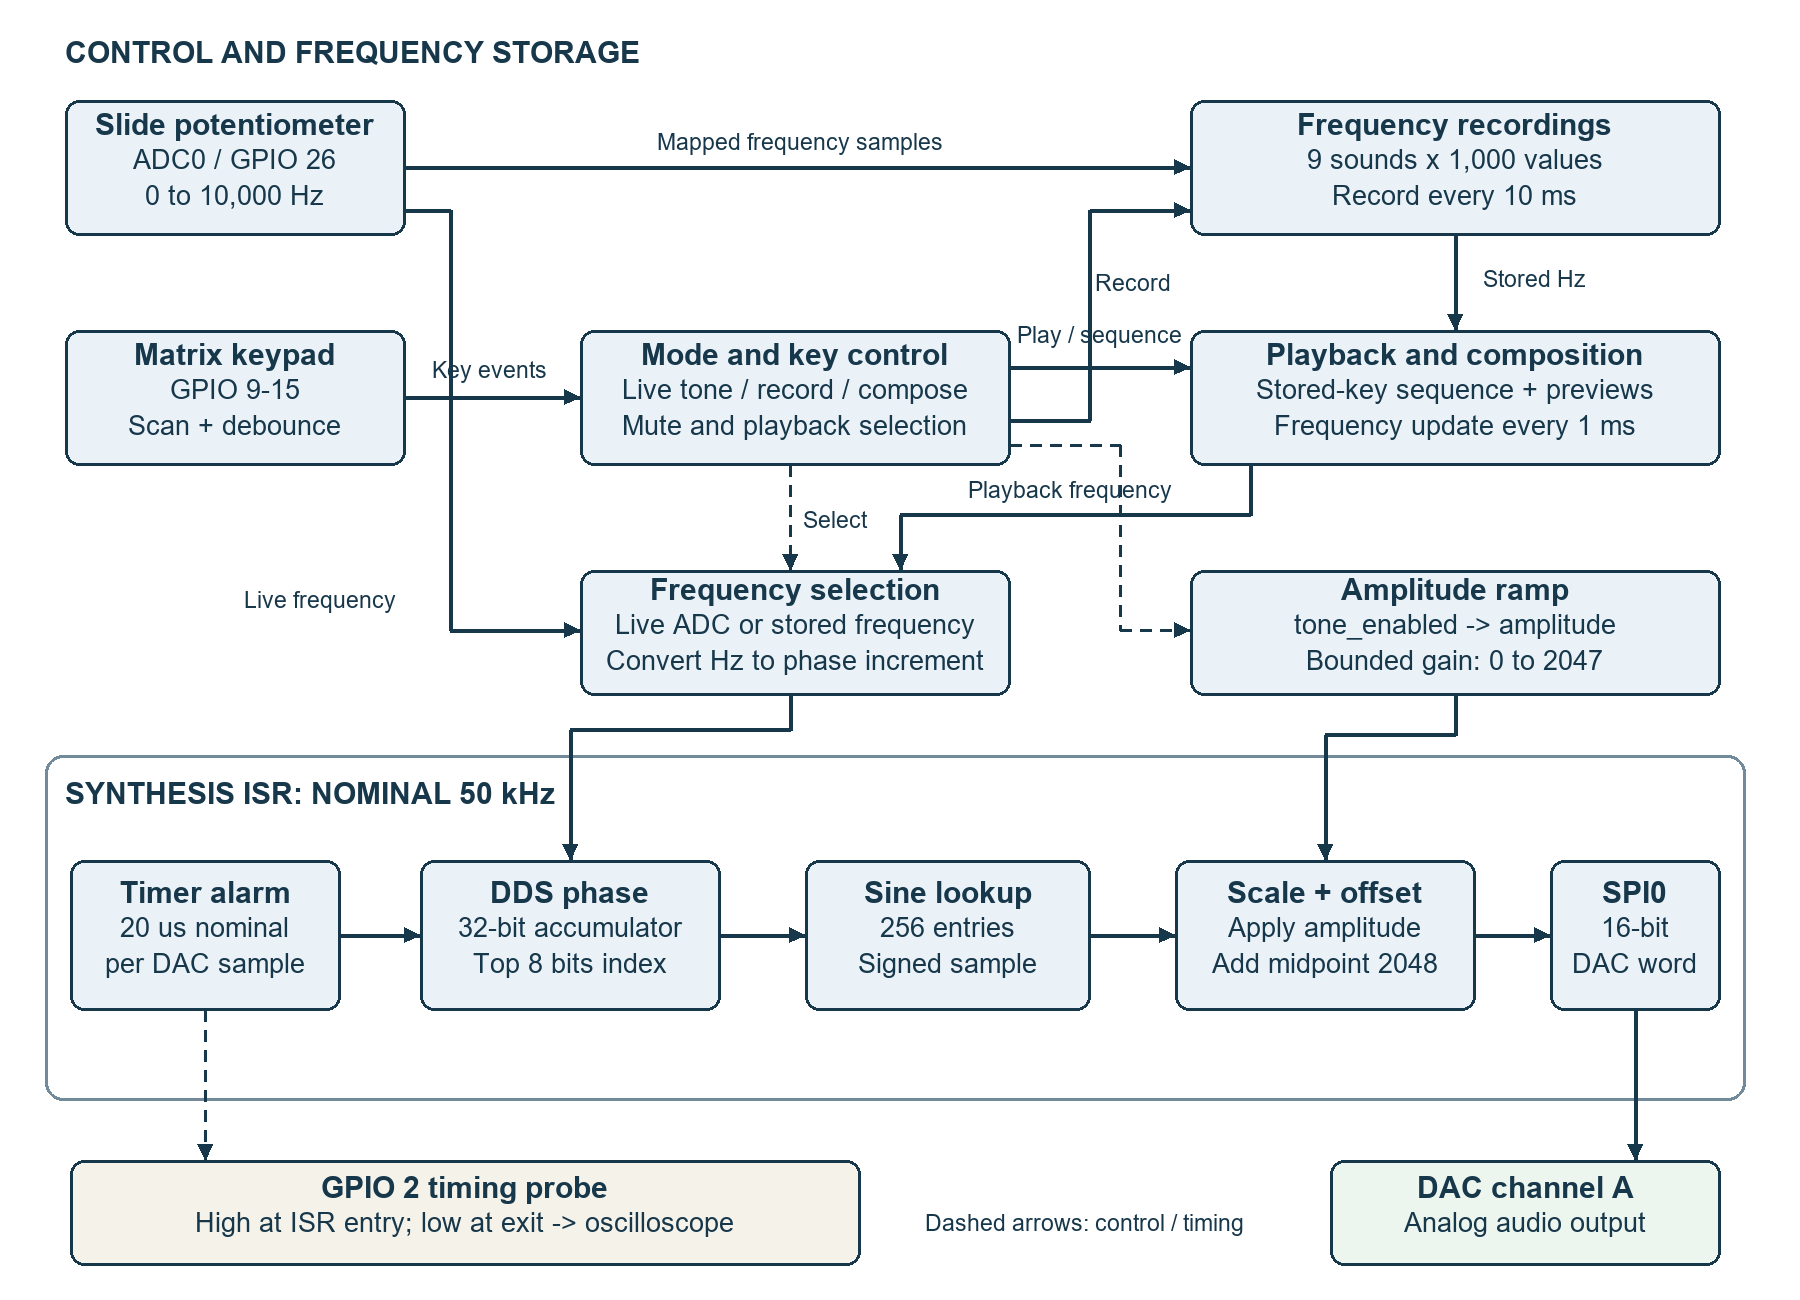
\includegraphics[width=\linewidth,height=0.65\textheight,keepaspectratio]{figures/signal_flow.png}
\caption{Functional signal flow derived from the saved implementation. Dashed arrows indicate control or timing signals; this is not an as-built wiring schematic.}
\end{figure}

\begingroup\small
\setlength{\tabcolsep}{5pt}
\begin{longtable}{|>{\raggedright\arraybackslash}p{0.295\linewidth}|>{\raggedright\arraybackslash}p{0.295\linewidth}|>{\raggedright\arraybackslash}p{0.295\linewidth}|}
\hline
\textbf{Pico signal} & \textbf{Program assignment} & \textbf{External connection / confirmation} \\ \hline
\endhead
GPIO 5 & SPI0 chip select & DAC active-low CS \\ \hline
GPIO 6 & SPI0 clock & DAC SCK \\ \hline
GPIO 7 & SPI0 transmit & DAC SDI \\ \hline
GPIO 4 & SPI0 receive function configured & No DAC read transaction is used \\ \hline
GPIO 26 & ADC0 & Potentiometer wiper \\ \hline
GPIO 9--12 & Row outputs & Keypad rows; confirm connector order \\ \hline
GPIO 13--15 & Pulled-up column inputs & Keypad columns; confirm connector order \\ \hline
GPIO 2 & ISR timing output & Scope probe \\ \hline
GPIO 25 & LED toggle output & Code assignment; board-specific LED behavior is not verification of audio \\ \hline
Supply and ground & Not established by C source & Add actual DAC, potentiometer, and shared-ground wiring \\ \hline
DAC latch, audio socket, boot button & Not established by C source & Add actual connections and any component values \\ \hline
\end{longtable}
\endgroup

\begin{figure}[H]
\centering
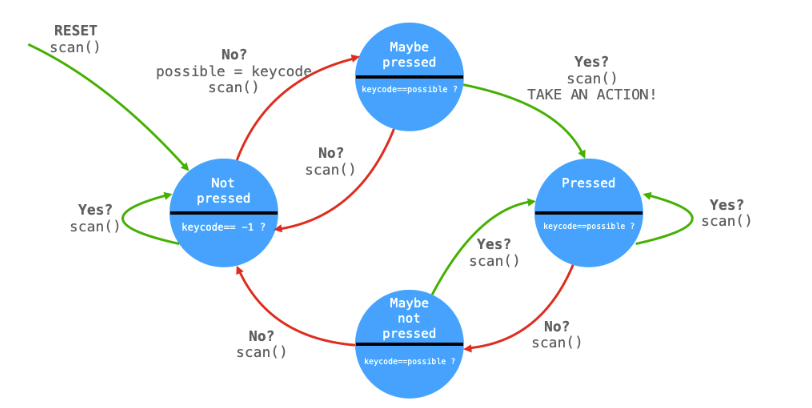
\includegraphics[width=\linewidth,height=0.65\textheight,keepaspectratio]{figures/debounce_state_machine.png}
\caption{Four-state keypad debounce diagram supplied by the group. The action on confirmed press matches the saved implementation; recording ends on confirmed release.}
\end{figure}

The keypad thread waits between scans, and each switch case ends with a break. This keeps one reading from moving through several states at once. The saved key value tells us which recording to stop after release. A different key also counts as losing the previous key, so this logic is meant for one key at a time.

\subsection*{3.2 Reproduction and program listings}

Our CMake target, \texttt{Audio\_Timer\_Interrupt\_DDS}, builds \texttt{ADC\_DDS\_keypad\_speedup.c} for \texttt{pico2}. The configuration lists SDK 2.3.0 and toolchain 15\_2\_Rel1. It also uses \texttt{pt\_cornell\_rp2040\_v1\_4.h}. To rebuild the project, keep the application file, protothreads header, SDK import file, and CMake setup together. Build with the Pico extension or CMake, then load the generated UF2 through the board's bootloader. These are the saved build settings, not a separate record of the tools used during checkout.

Appendix A contains the six C files and the CMake configuration. Extra comments explain the final program without changing its code. The file hashes identify the versions included here.

\section*{4. Results}

\subsection*{4.1 Source-derived performance}

\begingroup\small
\setlength{\tabcolsep}{5pt}
\begin{longtable}{|>{\raggedright\arraybackslash}p{0.295\linewidth}|>{\raggedright\arraybackslash}p{0.295\linewidth}|>{\raggedright\arraybackslash}p{0.295\linewidth}|}
\hline
\textbf{Quantity} & \textbf{Calculated or configured value} & \textbf{Interpretation} \\ \hline
\endhead
Audio sample rate & 50,000 samples/s nominal & Set by 20 \ensuremath{\mu}s alarm delay; actual period needs measurement \\ \hline
Frequency command range & 0--10,000 Hz & Integer mapping from ADC code \\ \hline
Mean frequency-command spacing & 10,000/4095 \ensuremath{\approx} 2.442 Hz per ADC code & Actual adjacent integer commands differ by 2 or 3 Hz \\ \hline
DDS increment resolution & 50,000/2\textasciicircum{}32 \ensuremath{\approx} 0.00001164 Hz & Ideal digital tuning granularity, not measured accuracy \\ \hline
Sine table & 256 entries & Phase index resolution 1.40625\ensuremath{^{\circ}} \\ \hline
Record interval & 10 ms nominal & Approximately 100 frequency entries/s \\ \hline
Playback interval & 1 ms nominal & Approximately 10\ensuremath{\times} trajectory speed \\ \hline
Per-key recording limit & 1,000 entries & Approximately 10 s recorded / 1 s accelerated \\ \hline
Frequency storage & 18,000 bytes & Nine arrays of 1,000 unsigned 16-bit values \\ \hline
Composition capacity & Nine entries & Repetitions allowed; no entry timestamps stored \\ \hline
Fade timescale & Approximately 1 ms & 20 updates with 50 \ensuremath{\mu}s yields; timing varies \\ \hline
SPI frame wire time & 16 / 20 MHz = 0.8 \ensuremath{\mu}s nominal & Excludes software and interrupt overhead \\ \hline
\end{longtable}
\endgroup

The ISR schedules the next alarm from the timer value it reads while running. Time spent entering the interrupt and reaching that line can therefore affect the real sample period. Since the DDS calculation assumes 50 kHz, a change in the sample rate also changes the output frequency. The thread delays are not exact deadlines either. Other work, including the frequency printout, can make updates late. This is why the timing values from the code are nominal rather than exact measurements.

\subsection*{4.2 Experimental observations}

\begingroup\small
\setlength{\tabcolsep}{5pt}
\begin{tabular}{|>{\raggedright\arraybackslash}p{0.295\linewidth}|>{\raggedright\arraybackslash}p{0.295\linewidth}|>{\raggedright\arraybackslash}p{0.295\linewidth}|}
\hline
\textbf{Measurement} & \textbf{Observed value} & \textbf{Evidence and interpretation} \\ \hline
Fixed-tone waveform & Scope displays 800.000 Hz & IMG\_7767; DAC output channel and instrument uncertainty not documented \\ \hline
Timing-pulse high interval & Cursor separation 1.63 \ensuremath{\mu}s & IMG\_7909; one capture, not a worst-case timing bound \\ \hline
Timing-trace repetition & Scope displays 50.0000 kHz, corresponding to 20.0 \ensuremath{\mu}s & IMG\_7909; period inferred from displayed frequency \\ \hline
Cardinal imitation / Merlin outcome & Northern Cardinal identified & Supplied Merlin screenshot and group demonstration account \\ \hline
\end{tabular}
\endgroup

The scope shows a sine wave at 800.000 Hz, with scales of 500 mV/division and 400 \ensuremath{\mu}s/division. That agrees with the 800 Hz test program. The photo does not identify which DAC output was probed. Also, the number of digits on the display does not tell us the measurement uncertainty, so we cannot claim zero frequency error.

\begin{figure}[H]
\centering
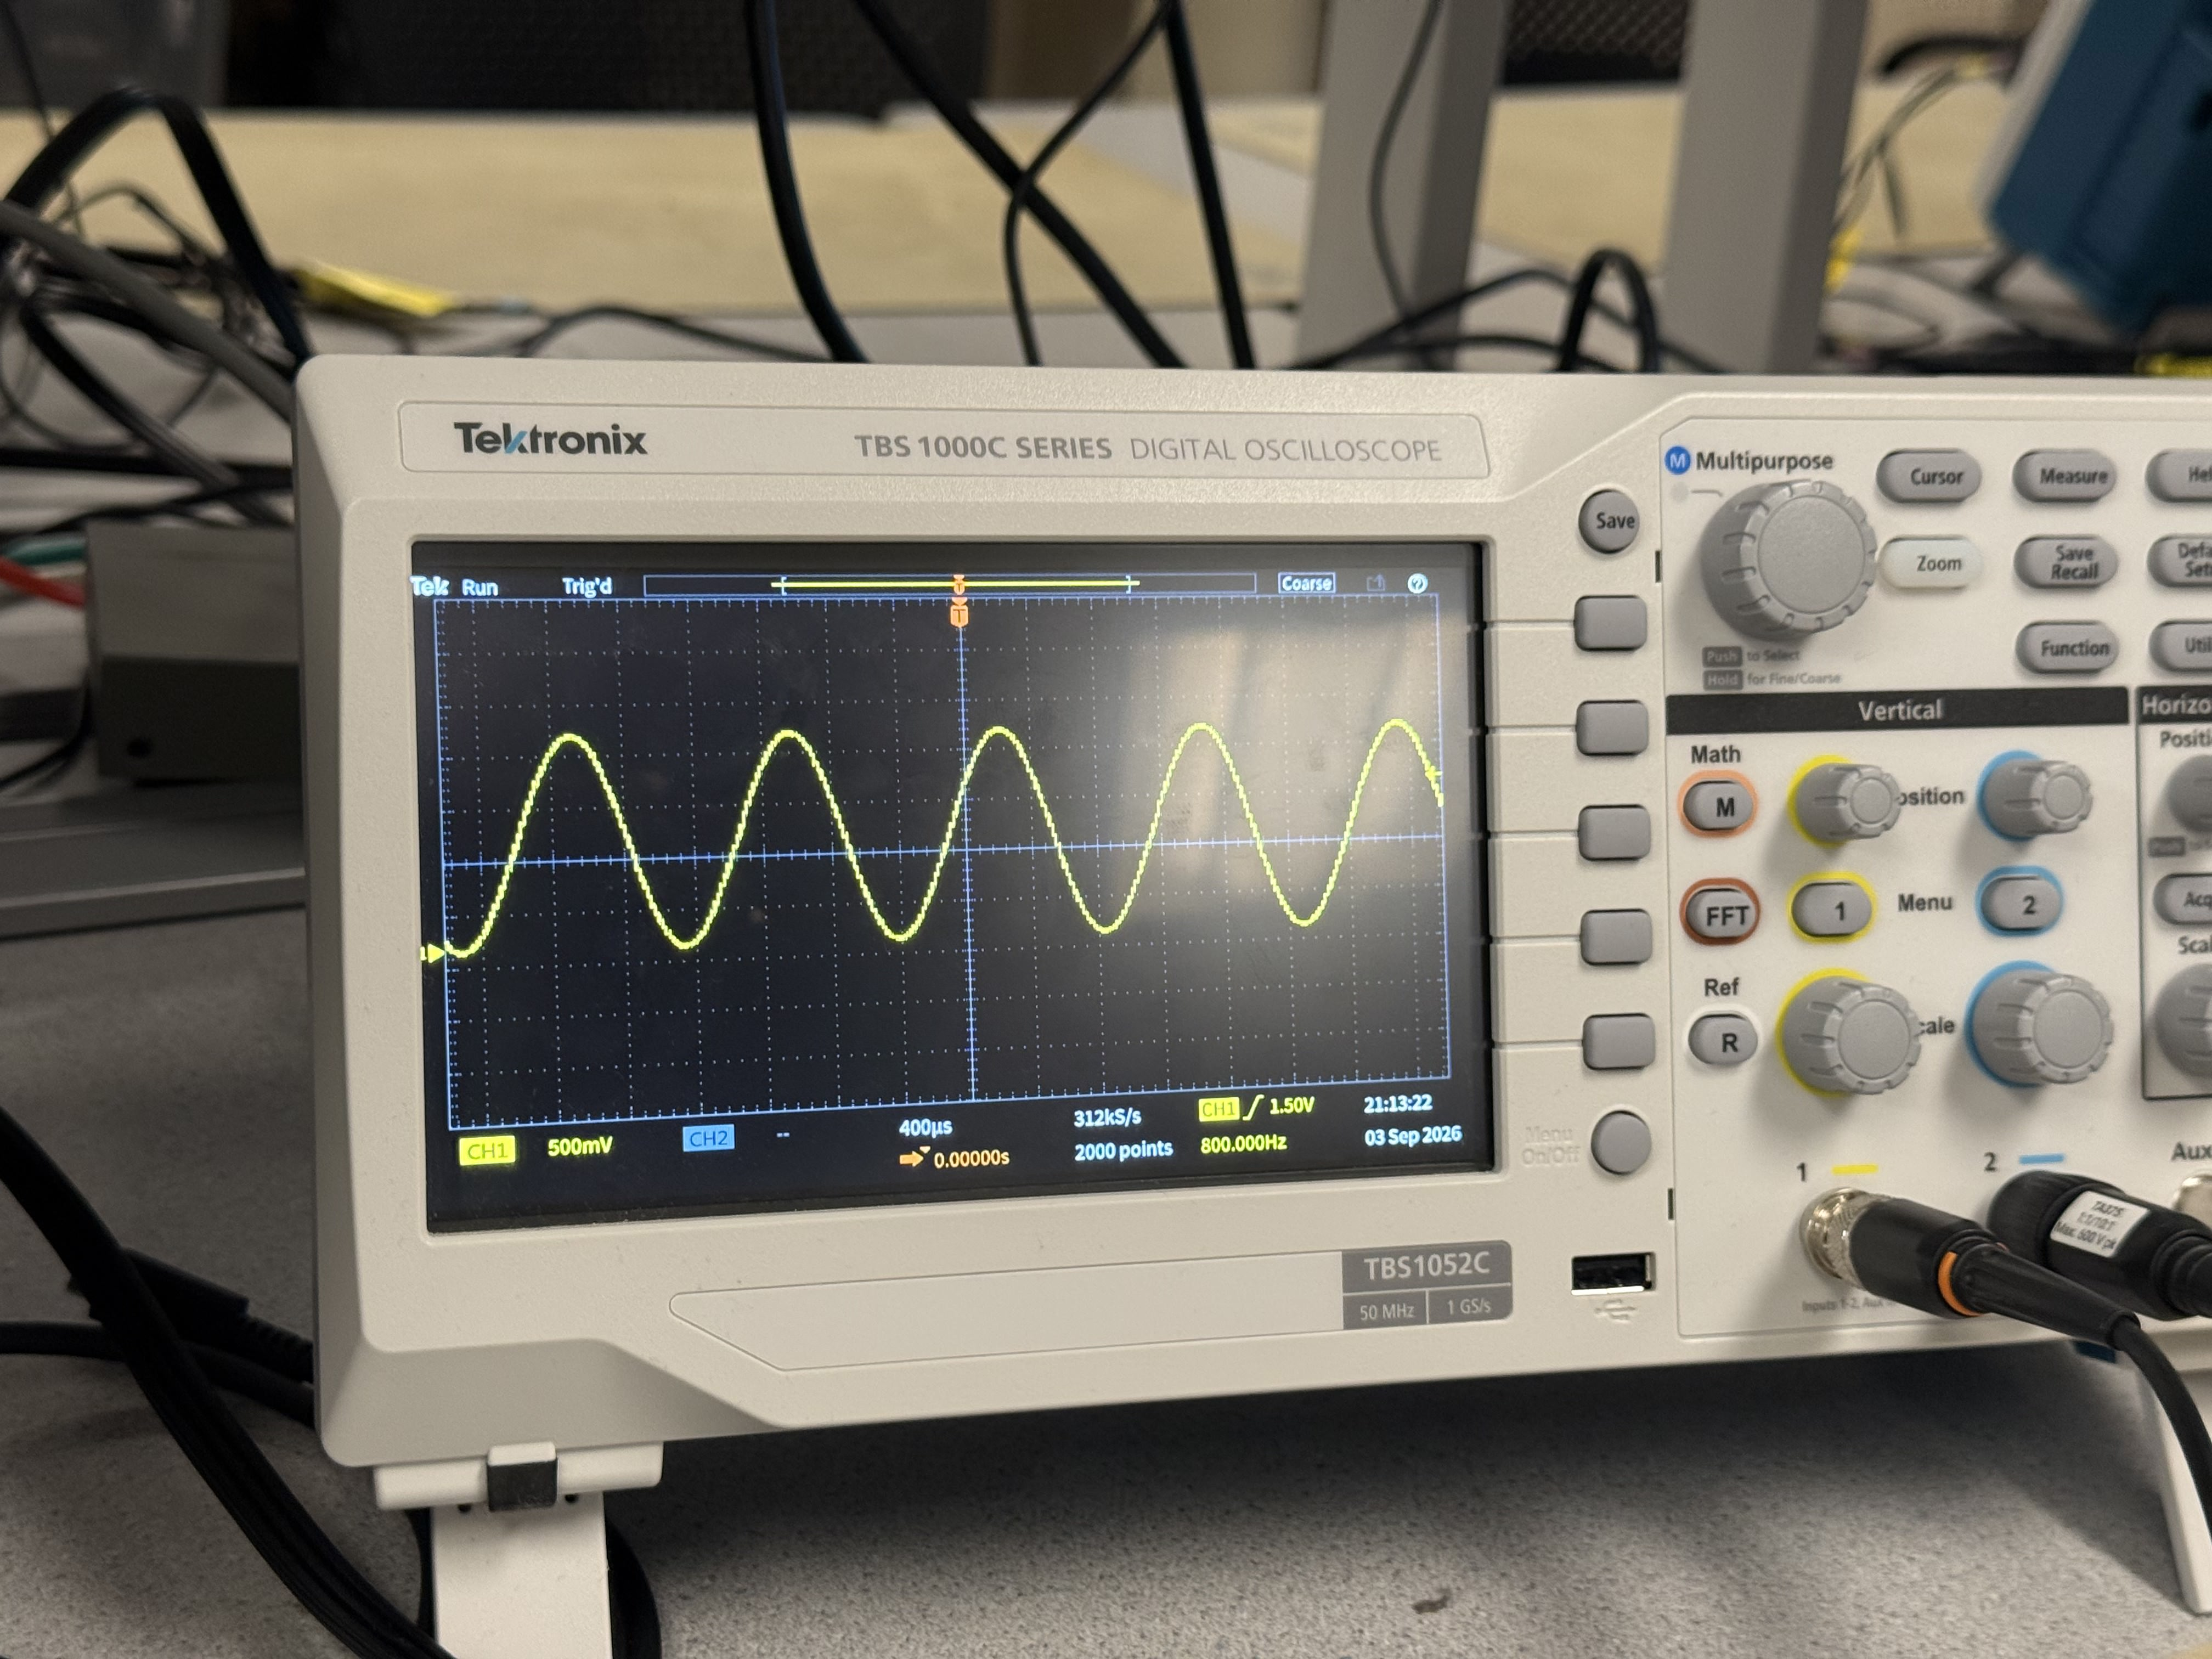
\includegraphics[width=\linewidth,height=0.65\textheight,keepaspectratio]{figures/tone_800hz.jpg}
\caption{Fixed-tone oscilloscope observation: sinusoidal output with an 800.000 Hz readout, 500 mV/division vertical scale, and 400 \ensuremath{\mu}s/division horizontal scale. Photograph: IMG\_7767.}
\end{figure}

The timing cursors are at about -48.0 ns and 1.58 \ensuremath{\mu}s, giving the displayed separation of 1.63 \ensuremath{\mu}s. The scope also shows 50.0000 kHz, or a 20.0 \ensuremath{\mu}s period. If this is the GPIO 2 timing signal, the measured part of the ISR uses about 1.63/20.0 = 8.15\% of each period. This matches the purpose of our timing code, though the photo does not show the probe connection or firmware version. It is one sample of the execution time, not a worst-case measurement, and it leaves out interrupt overhead before and after the GPIO writes.

\begin{figure}[H]
\centering
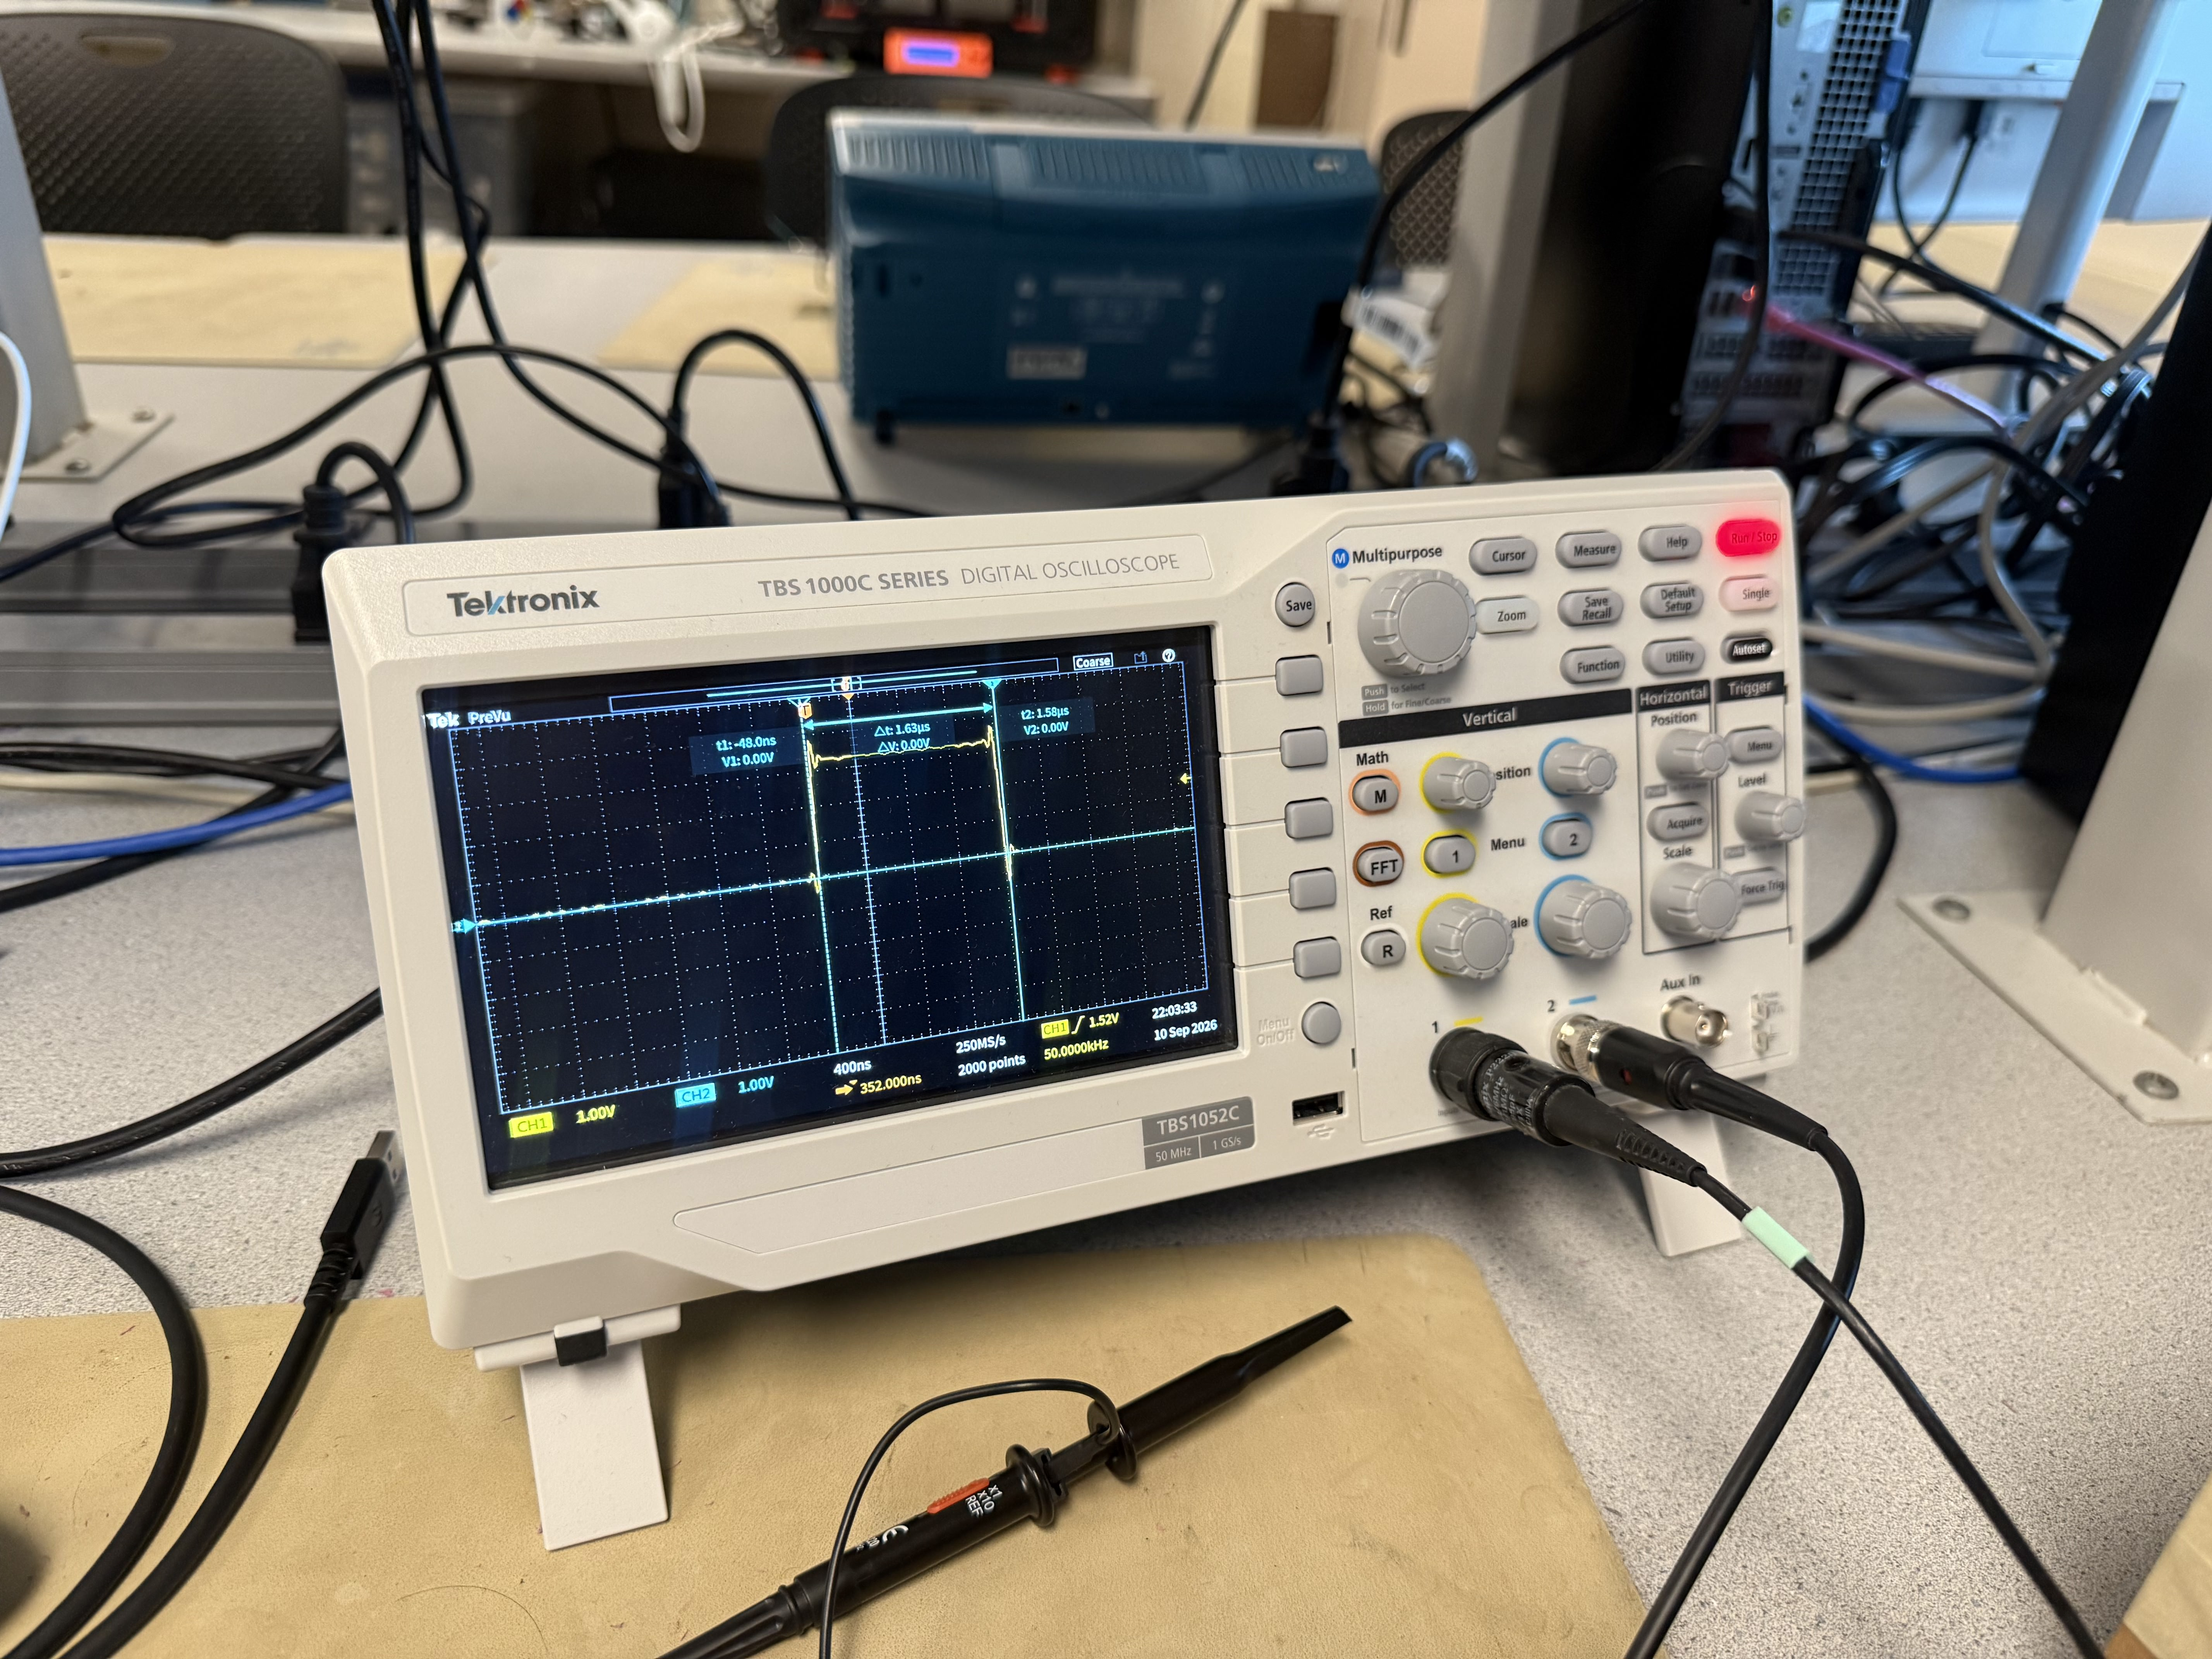
\includegraphics[width=\linewidth,height=0.65\textheight,keepaspectratio]{figures/isr_timing.jpg}
\caption{Timing-pulse oscilloscope capture with a 1.63 \ensuremath{\mu}s cursor separation and a 50.0000 kHz frequency readout. Horizontal scale: 400 ns/division. Photograph: IMG\_7909.}
\end{figure}

We do not have a scope capture showing a full sound's rise, sustain, and fall. The sine-wave photo shows the tone, but it does not replace the envelope capture requested in the lab.

Merlin listed Northern Cardinal under ``Best suggestions'' when we played our synthesized call. Its spectrogram is visible above the result. The screen shows September 10 in Ithaca, NY, with 00:56 of recording time. That timer belongs to the app; it is not the length of one call or a playback-speed measurement. The identification shows that Merlin recognized our sound as the intended bird, but the screenshot does not give a confidence score or enough axis information to measure spectral error.

\begin{figure}[H]
\centering
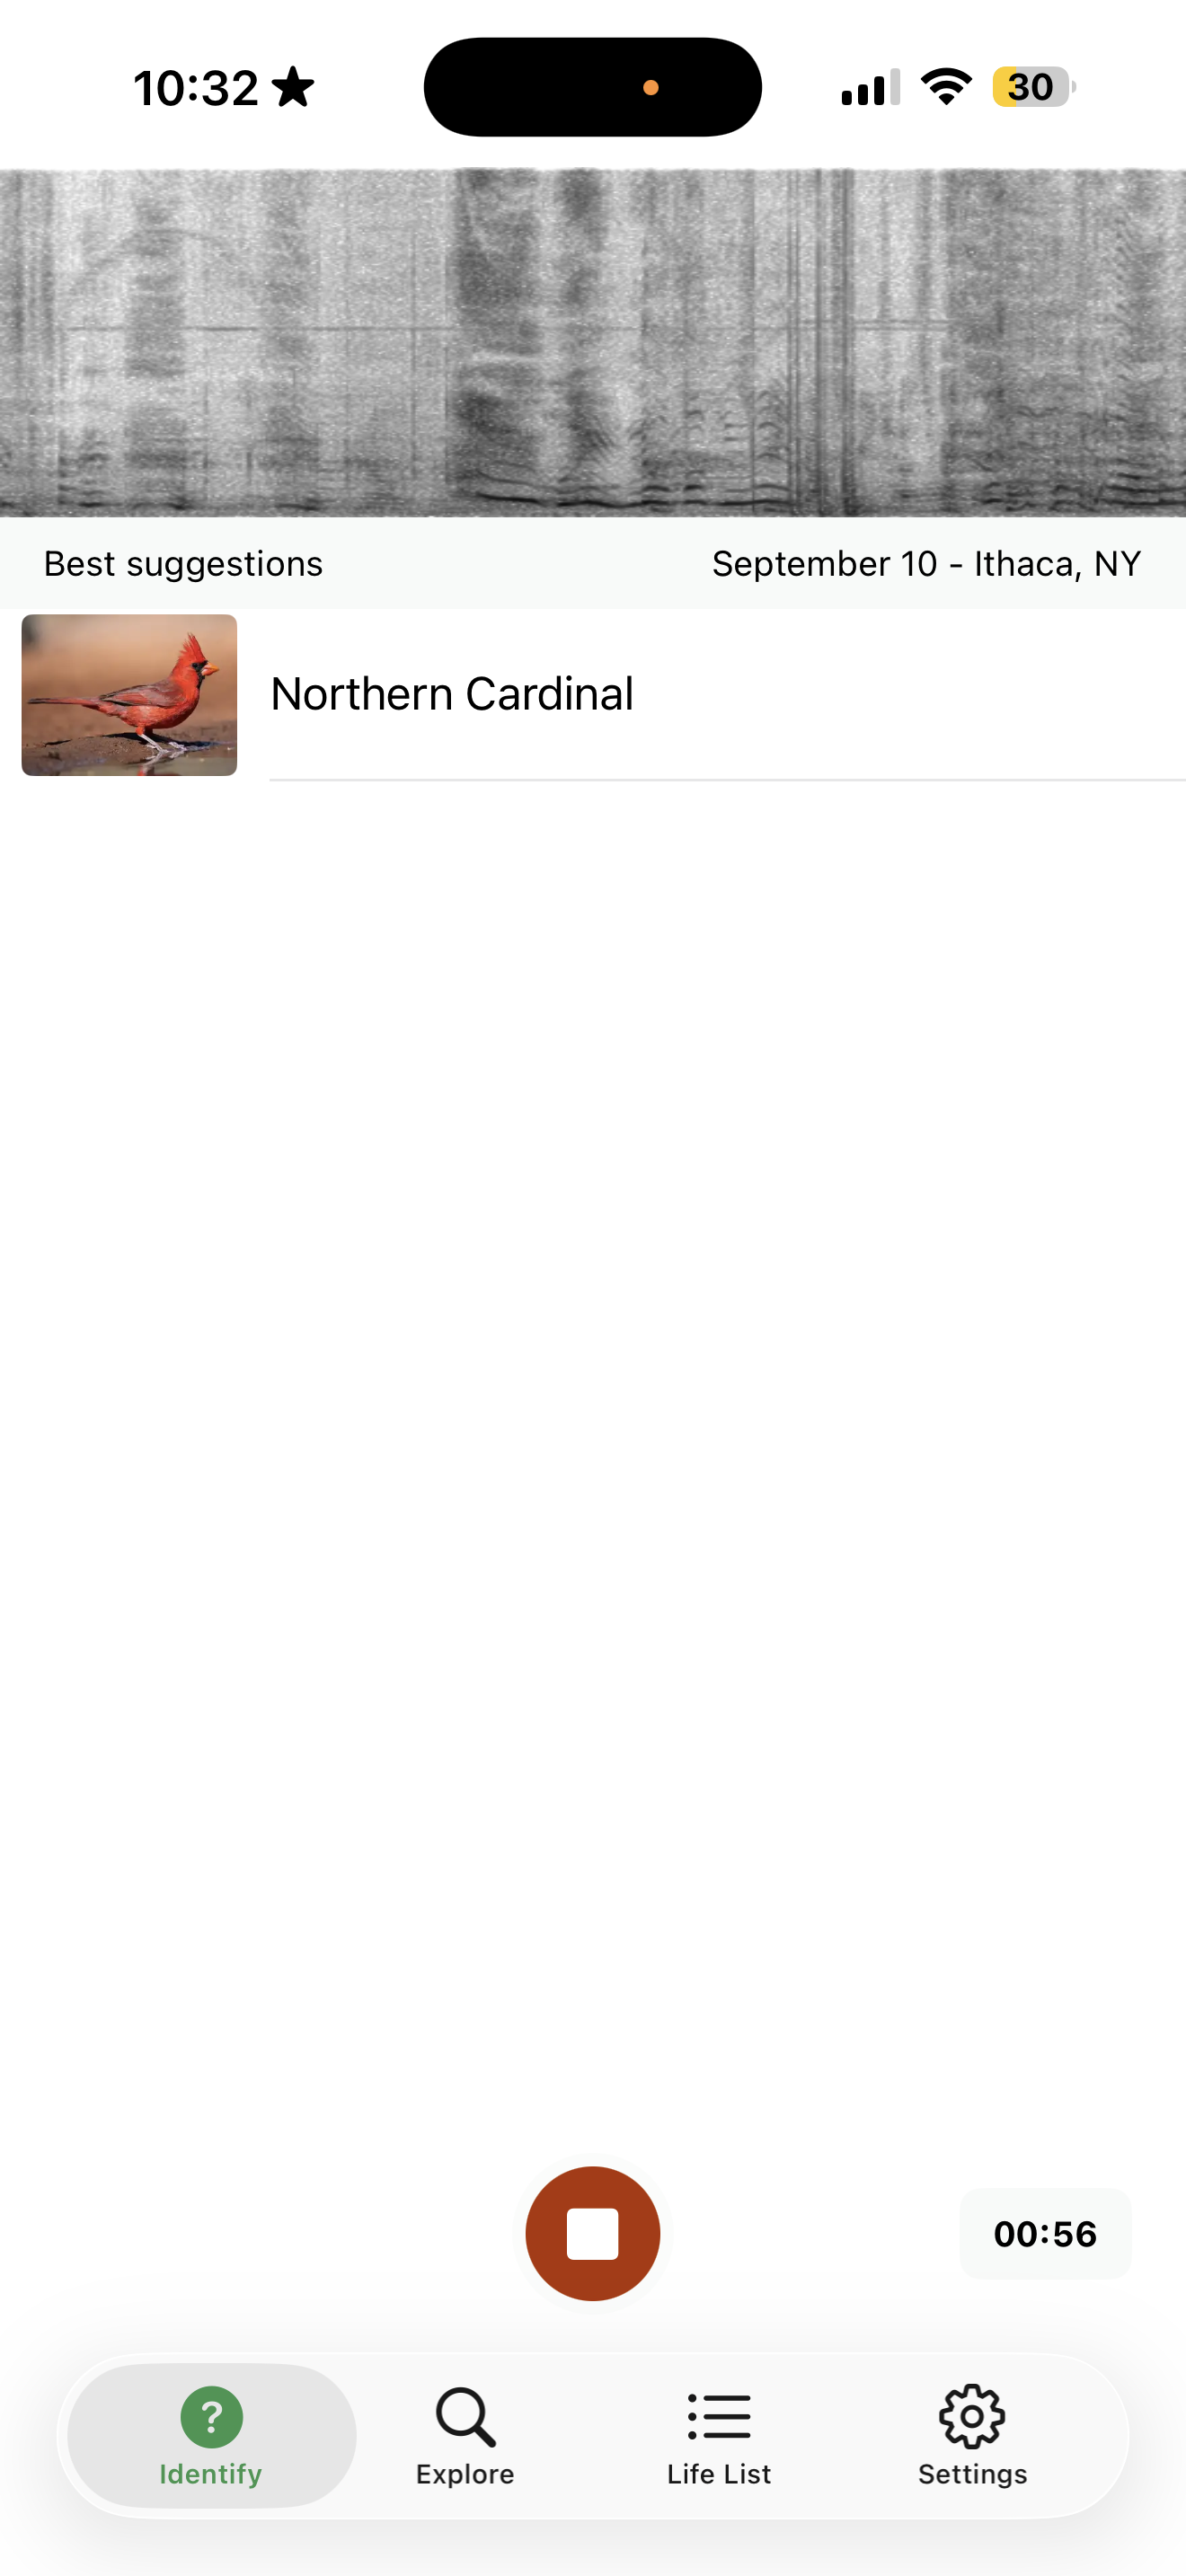
\includegraphics[width=0.70\linewidth,height=0.68\textheight,keepaspectratio]{figures/merlin_cardinal.png}
\caption{Merlin Sound ID identifies our synthesized birdsong as a Northern Cardinal. The live spectrogram is visible above the identification. Screenshot supplied by the group from the successful demonstration.}
\label{fig:merlin-cardinal}
\end{figure}

\subsection*{4.3 Limitations visible in the submitted snapshot}

There are still a few limits in the saved code. Most controls act on confirmed press, even though the comments describe release. Recording starts on the next held-key scan and ends after release is confirmed. A very short hold may not save anything. Since the old sound length is not cleared at the start, a recording with no new samples can leave the old sound in place.

Moving to the next sound in a composition takes a separate playback iteration. For about 1 ms, the previous frequency keeps playing. Empty sounds also take an iteration to skip, and an all-empty sequence can briefly play the previous frequency. We reject empty sounds for individual playback, but we still allow their key numbers into a composition. We also save only the key order, not the time between presses. Pausing while entering the sequence will not add a pause to playback.

The amplitude stays on between sounds in a composition, so each sound does not get its own fade in and fade out. At the end of playback, the ADC can take control of the frequency before the final fade has finished. These are possible sources of sound artifacts based on the code; we do not have measurements showing how audible they are.

\section*{5. Conclusions}

We combined a DDS tone generator with recording, faster playback, and a keypad interface for arranging sounds. Keeping earlier versions helped us track what we added each week. The sound previews make it easier to build a sequence, and key 0 gives us a way back to the potentiometer without resetting the board.

The main tradeoff was keeping the code simple while getting the timing right. Protothreads made the controls easier to organize, but a yield does not guarantee an exact update time. Fixed arrays were also straightforward to use, at the cost of limits on recording length and sequence size. If we extended the project, we would use one mode variable and shared functions for changing modes instead of resetting several flags in different places.

We would also schedule frequency updates against fixed deadlines, reduce the debug printing, and handle empty or full recordings more clearly. Giving each sound a defined envelope would improve transitions in a sequence. Our photos show the 800 Hz tone and a short timing pulse, and Merlin recognized the output as a Northern Cardinal. Those are useful results, but we did not measure worst-case ISR time or the exact playback-speed error.

\section*{6. Lab-Specific Deliverables and Questions}

The lab page does not list separate theory questions. It asks for an envelope scope capture, a spectrogram, commented code, and an AI prompt log with word and change counts. We included the tone and timing photos, Merlin's spectrogram, and the code in Appendix A. The envelope capture is missing. Appendix B contains the available prompt-log information and notes which counts still need the complete conversation. See the \href{https://vanhunteradams.com/Pico/Birds/Birdsong.html}{lab report instructions}.

Using the captured pulse, the measured portion of the ISR takes about 8.15 percent of the 20 microsecond period. This comes from \texttt{100 \ensuremath{\times} ISR\_high\_time / measured\_period} and does not include work outside the GPIO writes. Playback is nominally ten times faster because we read saved frequencies every 1 ms instead of every 10 ms. Storing frequency at 100 Hz also uses 1/500 as many entries as storing a waveform at 50 kHz, assuming the same number of bytes per entry.

We used the example reports as guides for organizing the design explanation, figures, results, and code appendix. Their measurements and results are not part of our data. References: \href{https://vanhunteradams.com/Pico/CourseMaterials/Birdsong.pdf}{Birdsong}, \href{https://vanhunteradams.com/Pico/CourseMaterials/Birdsong2.pdf}{Birdsong2}, \href{https://vanhunteradams.com/Pico/CourseMaterials/cricket.pdf}{Cricket}, and \href{https://vanhunteradams.com/Pico/CourseMaterials/reaction.pdf}{Reaction}.

\clearpage
\section*{Appendix A: Annotated Source Snapshot}

These files were saved on September 20, 2026. Comments marked REPORT NOTE explain the final code. They do not change how it runs; the other source text is unchanged.

\begingroup\small
\setlength{\tabcolsep}{5pt}
\begin{longtable}{|>{\raggedright\arraybackslash}p{0.458\linewidth}|>{\raggedright\arraybackslash}p{0.458\linewidth}|}
\hline
\textbf{File} & \textbf{SHA-256 of original bytes} \\ \hline
\endhead
dactest.c & \seqsplit{cc4bc1069280c53bd303e90ed557e279c2094c1c9d0648b568e8e1117b79701e} \\ \hline
dactest\_other\_channel.c & \seqsplit{db55fd5c39fc7d93591a67f3af02b89bf2e392f994765fd3cda78612e6356906} \\ \hline
ADC\_with\_DDS.c & \seqsplit{3fc01390cb1ba028b35a32cbb4d661edfecb50ade77d1f5c9b18ae416890af19} \\ \hline
ADC\_DDS\_keypad\_mute.c & \seqsplit{669d9393b6a637c8b51e0ce2d6ae9fc89231432dbc44c26fcb4d360034178846} \\ \hline
ADC\_DDS\_keypad\_record.c & \seqsplit{6ea0fd24342e753c004fb8e74a9a648411303fd9e9ab400118e07ef4037f6c55} \\ \hline
ADC\_DDS\_keypad\_speedup.c & \seqsplit{bb1a61ee89eeca9226ba5d9b1199d1cd2c6f6714c88119244d862d7483b6ac75} \\ \hline
CMakeLists.txt & \seqsplit{abbacbd8c017fe768584f6b78d768bbd91732b4158c4b4a4c254a1e04fd141c6} \\ \hline
\end{longtable}
\endgroup

\section*{dactest.c}

Week 1 baseline: a fixed 800 Hz phase increment feeds channel A. The timer ISR performs the table lookup and SPI write.

\begin{lstlisting}[language=C]
/**
 * V. Hunter Adams
 * DDS of sine wave on MCP4822 DAC w/ ISR
 * 
 * Modified example code from Raspberry Pi
 * Copyright (c) 2020 Raspberry Pi (Trading) Ltd.
 *
 * SPDX-License-Identifier: BSD-3-Clause
 *
   GPIO 5 (pin 7) Chip select
   GPIO 6 (pin 9) SCK/spi0_sclk
   GPIO 7 (pin 10) MOSI/spi0_tx
   GPIO 2 (pin 4) GPIO output for timing ISR
   3.3v (pin 36) -> VCC on DAC 
   GND (pin 3)  -> GND on DAC 
 */

#include <stdio.h>
#include <math.h>
#include "pico/stdlib.h"
#include "hardware/timer.h"
#include "hardware/irq.h"
#include "hardware/spi.h"

// Low-level alarm infrastructure we'll be using
#define ALARM_NUM 0
#define ALARM_IRQ timer_hardware_alarm_get_irq_num(timer_hw, ALARM_NUM)

//DDS parameters
#define two32 4294967296.0 // 2^32 
#define Fs 50000
#define DELAY 20 // 1/Fs (in microseconds)
// the DDS units:
volatile unsigned int phase_accum_main;
volatile unsigned int phase_incr_main = (800.0*two32)/Fs ;

// SPI data
uint16_t DAC_data ; // output value

//DAC parameters
// A-channel, 1x, active
#define DAC_config_chan_A 0b0011000000000000
// B-channel, 1x, active
#define DAC_config_chan_B 0b1011000000000000

//SPI configurations
#define PIN_MISO 4
#define PIN_CS   5
#define PIN_SCK  6
#define PIN_MOSI 7
#define SPI_PORT spi0

//GPIO for timing the ISR
#define ISR_GPIO 2

// DDS sine table
#define sine_table_size 256
volatile int sin_table[sine_table_size] ;

// Alarm ISR
static void alarm_irq(void) {

    // Assert a GPIO when we enter the interrupt
    gpio_put(ISR_GPIO, 1) ;

    // Clear the alarm irq
    hw_clear_bits(&timer_hw->intr, 1u << ALARM_NUM);

    // Reset the alarm register
    timer_hw->alarm[ALARM_NUM] = timer_hw->timerawl + DELAY ;

	// DDS phase and sine table lookup
	phase_accum_main += phase_incr_main  ;
    DAC_data = (DAC_config_chan_A | ((sin_table[phase_accum_main>>24] + 2048) & 0xffff))  ;

    // Perform an SPI transaction
    spi_write16_blocking(SPI_PORT, &DAC_data, 1) ;

    // De-assert the GPIO when we leave the interrupt
    gpio_put(ISR_GPIO, 0) ;

}

int main() {
    // Initialize stdio
    stdio_init_all();
    printf("Hello, DAC!\n");

    // Initialize SPI channel (channel, baud rate set to 20MHz)
    spi_init(SPI_PORT, 20000000) ;
    // Format (channel, data bits per transfer, polarity, phase, order)
    spi_set_format(SPI_PORT, 16, 0, 0, 0);

    // Setup the ISR-timing GPIO
    gpio_init(ISR_GPIO) ;
    gpio_set_dir(ISR_GPIO, GPIO_OUT);
    gpio_put(ISR_GPIO, 0) ;

    // Map SPI signals to GPIO ports
    gpio_set_function(PIN_MISO, GPIO_FUNC_SPI);
    gpio_set_function(PIN_SCK, GPIO_FUNC_SPI);
    gpio_set_function(PIN_MOSI, GPIO_FUNC_SPI);
    gpio_set_function(PIN_CS, GPIO_FUNC_SPI) ;

    // === build the sine lookup table =======
   	// scaled to produce values between 0 and 4096
    int ii;
    for (ii = 0; ii < sine_table_size; ii++){
         sin_table[ii] = (int)(2047*sin((float)ii*6.283/(float)sine_table_size));
    }

    // Enable the interrupt for the alarm (we're using Alarm 0)
    hw_set_bits(&timer_hw->inte, 1u << ALARM_NUM) ;
    // Associate an interrupt handler with the ALARM_IRQ
    irq_set_exclusive_handler(ALARM_IRQ, alarm_irq) ;
    // Enable the alarm interrupt
    irq_set_enabled(ALARM_IRQ, true) ;
    // Write the lower 32 bits of the target time to the alarm register, arming it.
    timer_hw->alarm[ALARM_NUM] = timer_hw->timerawl + DELAY ;

    // Nothing happening here
    while(1){
    }
    return 0;
}
\end{lstlisting}


\section*{dactest\_other\_channel.c}

Week 1 channel experiment: the DAC control word selects B rather than A. The DDS frequency remains 800 Hz.

\begin{lstlisting}[language=C]
/**
 * V. Hunter Adams
 * DDS of sine wave on MCP4822 DAC w/ ISR
 * 
 * Modified example code from Raspberry Pi
 * Copyright (c) 2020 Raspberry Pi (Trading) Ltd.
 *
 * SPDX-License-Identifier: BSD-3-Clause
 *
   GPIO 5 (pin 7) Chip select
   GPIO 6 (pin 9) SCK/spi0_sclk
   GPIO 7 (pin 10) MOSI/spi0_tx
   GPIO 2 (pin 4) GPIO output for timing ISR
   3.3v (pin 36) -> VCC on DAC 
   GND (pin 3)  -> GND on DAC 
 */

#include <stdio.h>
#include <math.h>
#include "pico/stdlib.h"
#include "hardware/timer.h"
#include "hardware/irq.h"
#include "hardware/spi.h"

// Low-level alarm infrastructure we'll be using
#define ALARM_NUM 0
#define ALARM_IRQ timer_hardware_alarm_get_irq_num(timer_hw, ALARM_NUM)

//DDS parameters
#define two32 4294967296.0 // 2^32 
#define Fs 50000
#define DELAY 20 // 1/Fs (in microseconds)
// the DDS units:
volatile unsigned int phase_accum_main;
volatile unsigned int phase_incr_main = (800.0*two32)/Fs ;

// SPI data
uint16_t DAC_data ; // output value

//DAC parameters
// A-channel, 1x, active
#define DAC_config_chan_A 0b0011000000000000
// B-channel, 1x, active
#define DAC_config_chan_B 0b1011000000000000

//SPI configurations
#define PIN_MISO 4
#define PIN_CS   5
#define PIN_SCK  6
#define PIN_MOSI 7
#define SPI_PORT spi0

//GPIO for timing the ISR
#define ISR_GPIO 2

// DDS sine table
#define sine_table_size 256
volatile int sin_table[sine_table_size] ;

// Alarm ISR
static void alarm_irq(void) {

    // Assert a GPIO when we enter the interrupt
    gpio_put(ISR_GPIO, 1) ;

    // Clear the alarm irq
    hw_clear_bits(&timer_hw->intr, 1u << ALARM_NUM);

    // Reset the alarm register
    timer_hw->alarm[ALARM_NUM] = timer_hw->timerawl + DELAY ;

	// DDS phase and sine table lookup
	phase_accum_main += phase_incr_main  ;
    DAC_data = (DAC_config_chan_B | ((sin_table[phase_accum_main>>24] + 2048) & 0xffff))  ;

    // Perform an SPI transaction
    spi_write16_blocking(SPI_PORT, &DAC_data, 1) ;

    // De-assert the GPIO when we leave the interrupt
    gpio_put(ISR_GPIO, 0) ;

}

int main() {
    // Initialize stdio
    stdio_init_all();
    printf("Hello, DAC!\n");

    // Initialize SPI channel (channel, baud rate set to 20MHz)
    spi_init(SPI_PORT, 20000000) ;
    // Format (channel, data bits per transfer, polarity, phase, order)
    spi_set_format(SPI_PORT, 16, 0, 0, 0);

    // Setup the ISR-timing GPIO
    gpio_init(ISR_GPIO) ;
    gpio_set_dir(ISR_GPIO, GPIO_OUT);
    gpio_put(ISR_GPIO, 0) ;

    // Map SPI signals to GPIO ports
    gpio_set_function(PIN_MISO, GPIO_FUNC_SPI);
    gpio_set_function(PIN_SCK, GPIO_FUNC_SPI);
    gpio_set_function(PIN_MOSI, GPIO_FUNC_SPI);
    gpio_set_function(PIN_CS, GPIO_FUNC_SPI) ;

    // === build the sine lookup table =======
   	// scaled to produce values between 0 and 4096
    int ii;
    for (ii = 0; ii < sine_table_size; ii++){
         sin_table[ii] = (int)(2047*sin((float)ii*6.283/(float)sine_table_size));
    }

    // Enable the interrupt for the alarm (we're using Alarm 0)
    hw_set_bits(&timer_hw->inte, 1u << ALARM_NUM) ;
    // Associate an interrupt handler with the ALARM_IRQ
    irq_set_exclusive_handler(ALARM_IRQ, alarm_irq) ;
    // Enable the alarm interrupt
    irq_set_enabled(ALARM_IRQ, true) ;
    // Write the lower 32 bits of the target time to the alarm register, arming it.
    timer_hw->alarm[ALARM_NUM] = timer_hw->timerawl + DELAY ;

    // Nothing happening here
    while(1){
    }
    return 0;
}
\end{lstlisting}


\section*{ADC\_with\_DDS.c}

Week 1 integration: the ADC thread converts a potentiometer code to Hz, then to a phase increment. The timer ISR independently emits audio samples.

\begin{lstlisting}[language=C]

/*
Simple ADC/Protothreads demo

Schedules a single thread, reads/prints ADC value

 */

#include "hardware/gpio.h"
#include "hardware/timer.h"
#include "hardware/adc.h"
#include "pico/stdlib.h"
#include <stdio.h>
#include <string.h>
#include "stdlib.h"
#include "hardware/spi.h"
#include <math.h>
#include "hardware/irq.h"

// ==========================================
// === protothreads globals
// ==========================================
// protothreads header
#include "pt_cornell_rp2040_v1_4.h"

#define LED_PIN 25
#define ADC_PIN 26
#define ADC_MUX 0

// Low-level alarm infrastructure we'll be using
#define ALARM_NUM 0
#define ALARM_IRQ timer_hardware_alarm_get_irq_num(timer_hw, ALARM_NUM)

//DDS parameters
#define two32 4294967296.0 // 2^32 
#define Fs 50000
#define DELAY 20 // 1/Fs (in microseconds)
// the DDS units:
volatile unsigned int phase_accum_main;
volatile unsigned int phase_incr_main;

// SPI data
uint16_t DAC_data ; // output value

//DAC parameters
// A-channel, 1x, active
#define DAC_config_chan_A 0b0011000000000000
// B-channel, 1x, active
#define DAC_config_chan_B 0b1011000000000000

//SPI configurations
#define PIN_MISO 4
#define PIN_CS   5
#define PIN_SCK  6
#define PIN_MOSI 7
#define SPI_PORT spi0

//GPIO for timing the ISR
#define ISR_GPIO 2

// DDS sine table
#define sine_table_size 256
volatile int sin_table[sine_table_size] ;

volatile static unsigned int adc_val ;

static int map(int x, int in_min, int in_max, int out_min, int out_max) {
    return (x - in_min) * (out_max - out_min) / (in_max - in_min) + out_min;
}

// ==================================================
// === toggle25 thread 
// ==================================================
//  
static PT_THREAD (protothread_toggle25(struct pt *pt))
{
    PT_BEGIN(pt);

      while(1) {
        // toggle gpio 25
        gpio_put(LED_PIN, !gpio_get(LED_PIN));

        // Read the ADC
        adc_val = adc_read() ;

        phase_incr_main = (map(adc_val, 0, 4095, 0, 10000)*two32)/Fs;

        // Print the value
        printf("ADC value: %d\n", adc_val) ;

        // Yield
        PT_YIELD_usec(10000) ; //yeild every 10 ms
      } // END WHILE(1)
      // every thread ends with PT_END(pt);
      PT_END(pt);
} // end blink thread

// Alarm ISR
static void alarm_irq(void) {

    // Assert a GPIO when we enter the interrupt
    gpio_put(ISR_GPIO, 1) ;

    // Clear the alarm irq
    hw_clear_bits(&timer_hw->intr, 1u << ALARM_NUM);

    // Reset the alarm register
    timer_hw->alarm[ALARM_NUM] = timer_hw->timerawl + DELAY ; 

    // DDS phase and sine table lookup
    phase_accum_main += phase_incr_main  ;
    DAC_data = (DAC_config_chan_A | ((sin_table[phase_accum_main>>24] + 2048) & 0xffff))  ;

    // Perform an SPI transaction
    spi_write16_blocking(SPI_PORT, &DAC_data, 1) ;

    // De-assert the GPIO when we leave the interrupt
    gpio_put(ISR_GPIO, 0) ;

}

// ========================================
// === core 0 main
// ========================================
int main(){
  //===  start the serial i/o ==================
  stdio_init_all() ;
  // announce the threader version on system reset
  // if there is a seral terminal attached
  printf("\n\rProtothreads RP2040 v1.4\n\r");

  // Setup the ADC
  adc_init() ;
  adc_gpio_init(ADC_PIN) ;
  adc_select_input(ADC_MUX) ;

  // Initialize stdio
    stdio_init_all();
    printf("Hello, DAC!\n");

    // Initialize SPI channel (channel, baud rate set to 20MHz)
    spi_init(SPI_PORT, 20000000) ;
    // Format (channel, data bits per transfer, polarity, phase, order)
    spi_set_format(SPI_PORT, 16, 0, 0, 0);

    // Setup the ISR-timing GPIO
    gpio_init(ISR_GPIO) ;
    gpio_set_dir(ISR_GPIO, GPIO_OUT);
    gpio_put(ISR_GPIO, 0) ;

    // Map SPI signals to GPIO ports
    gpio_set_function(PIN_MISO, GPIO_FUNC_SPI);
    gpio_set_function(PIN_SCK, GPIO_FUNC_SPI);
    gpio_set_function(PIN_MOSI, GPIO_FUNC_SPI);
    gpio_set_function(PIN_CS, GPIO_FUNC_SPI) ;

    // === build the sine lookup table =======
   	// scaled to produce values between 0 and 4096
    int ii;
    for (ii = 0; ii < sine_table_size; ii++){
         sin_table[ii] = (int)(2047*sin((float)ii*6.283/(float)sine_table_size));
    }

        // Enable the interrupt for the alarm (we're using Alarm 0)
    hw_set_bits(&timer_hw->inte, 1u << ALARM_NUM) ;
    // Associate an interrupt handler with the ALARM_IRQ
    irq_set_exclusive_handler(ALARM_IRQ, alarm_irq) ;
    // Enable the alarm interrupt
    irq_set_enabled(ALARM_IRQ, true) ;
    // Write the lower 32 bits of the target time to the alarm register, arming it.
    timer_hw->alarm[ALARM_NUM] = timer_hw->timerawl + DELAY ;

  // set up LED gpio 25
  gpio_init(LED_PIN) ;  
  gpio_set_dir(LED_PIN, GPIO_OUT) ;
  gpio_put(LED_PIN, true);

  // === config threads ========================
  pt_add_thread(protothread_toggle25);
  
  // === initalize the scheduler ===============
  pt_schedule_start ;

    // Nothing happening here
    while(1){
    }
    return 0;
} // end main
\end{lstlisting}


\section*{ADC\_DDS\_keypad\_mute.c}

Week 2 mute stage: keypad scanning and a four-state debounce machine set tone\_enabled; the amplitude thread ramps output rather than rebuilding the sine table.

\begin{lstlisting}[language=C]

/*
Simple ADC/Protothreads demo

Schedules a single thread, reads/prints ADC value

 */

#include "hardware/gpio.h"
#include "hardware/timer.h"
#include "hardware/adc.h"
#include "pico/stdlib.h"
#include "pico/multicore.h"
#include <stdio.h>
#include <string.h>
#include "stdlib.h"
#include "hardware/spi.h"
#include <math.h>
#include "hardware/irq.h"
#include "hardware/pio.h"
#include "hardware/dma.h"
#include "hardware/sync.h"
#include "hardware/spi.h"
#include "hardware/clocks.h"

// ==========================================
// === protothreads globals
// ==========================================
// protothreads header
#include "pt_cornell_rp2040_v1_4.h"

#define LED_PIN 25
#define ADC_PIN 26
#define ADC_MUX 0

// Low-level alarm infrastructure we'll be using
#define ALARM_NUM 0
#define ALARM_IRQ timer_hardware_alarm_get_irq_num(timer_hw, ALARM_NUM)

//DDS parameters
#define two32 4294967296.0 // 2^32 
#define Fs 50000
#define DELAY 20 // 1/Fs (in microseconds)

//keypad constants
#define BASE_KEYPAD_PIN 9
#define KEYROWS         4
#define NUMKEYS         12
// the DDS units:
volatile unsigned int phase_accum_main;
volatile unsigned int phase_incr_main;

// SPI data
uint16_t DAC_data ; // output value

//DAC parameters
// A-channel, 1x, active
#define DAC_config_chan_A 0b0011000000000000
// B-channel, 1x, active
#define DAC_config_chan_B 0b1011000000000000

//SPI configurations
#define PIN_MISO 4
#define PIN_CS   5
#define PIN_SCK  6
#define PIN_MOSI 7
#define SPI_PORT spi0

//GPIO for timing the ISR
#define ISR_GPIO 2

// DDS sine table
#define sine_table_size 256
volatile int sin_table[sine_table_size] ;

volatile static unsigned int adc_val ;

static int map(int x, int in_min, int in_max, int out_min, int out_max) {
    return (x - in_min) * (out_max - out_min) / (in_max - in_min) + out_min;
}

//keycodes
unsigned int keycodes[NUMKEYS] = {      0x57, 0x6E, 0x5E, 0x3E, 0x6D,
                                        0x5D, 0x3D, 0x6B, 0x5B, 0x3B,
                                        0x67, 0x37} ;
unsigned int scancodes[KEYROWS] = {   0xE, 0xD, 0xB, 0x7} ;
unsigned int button = 0x70 ;
char keytext[40];
int prev_key = 0;

//muting variables
#define AMPLITUDE_STEP 103 // 20 updates at 1 ms each for a full fade
volatile bool tone_enabled = true;
volatile int amplitude = 2047; // 0 = silent, 2047 = full amplitude

//debouncing states
#define NOT_PRESSED 0
#define MAYBE_PRESSED 1
#define PRESSED 2
#define MAYBE_NOT_PRESSED 3


// ==================================================
// === toggle25 thread 
// ==================================================
//  
static PT_THREAD (protothread_toggle25(struct pt *pt))
{
    PT_BEGIN(pt);

      while(1) {
        // toggle gpio 25
        gpio_put(LED_PIN, !gpio_get(LED_PIN));

        // Read the ADC
        adc_val = adc_read() ;

        phase_incr_main = (map(adc_val, 0, 4095, 0, 10000)*two32)/Fs;

        // Print the value
        printf("ADC value: %d\n", adc_val) ;

        // Yield
        PT_YIELD_usec(10000) ; //yeild every 10 ms
      } // END WHILE(1)
      // every thread ends with PT_END(pt);
      PT_END(pt);
} // end blink thread

// This thread runs on core 0
static PT_THREAD (protothread_core_0(struct pt *pt))
{
    // Indicate thread beginning
    PT_BEGIN(pt) ;

    // Some variables
    static int i ;
    static uint32_t keypad ;
    static int possible;
    static int state;

    while(1) {

        // Scan the keypad!
        for (i=0; i<KEYROWS; i++) {
            // Set a row high
            gpio_put_masked((0xF << BASE_KEYPAD_PIN),
                            (scancodes[i] << BASE_KEYPAD_PIN)) ;
            // Small delay required
            sleep_us(1) ;
            // Read the keycode
            keypad = ((gpio_get_all() >> BASE_KEYPAD_PIN) & 0x7F) ;
            // Break if button(s) are pressed
            if ((~keypad) & button) break ;
        }
        // If we found a button . . .
        if ((~keypad) & button) {
            // Look for a valid keycode.
            for (i=0; i<NUMKEYS; i++) {
                if (keypad == keycodes[i]) break ;
            }
            // If we don't find one, report invalid keycode
            if (i==NUMKEYS) (i = -1) ;
        }
        // Otherwise, indicate invalid/non-pressed buttons
        else (i=-1) ;

        switch (state) {

          case NOT_PRESSED:
            if (i != -1) {
              possible = i;
              state = MAYBE_PRESSED;
            }
            break;

          case MAYBE_PRESSED:
            if (i == possible){
              state = PRESSED;
              // Toggle once on confirmed release of the remembered key.
              if (possible == 0) {
                tone_enabled = !tone_enabled;
              // Print key to terminal
              printf("\n%d", i) ;
              }
            }
            else {
              state = NOT_PRESSED;
            }
            break;
          
          case PRESSED:
            if (i == possible){
              state = PRESSED;
            }
            else {
              state = MAYBE_NOT_PRESSED;
            }
            break;

          case MAYBE_NOT_PRESSED:
            if (i == possible){
              state = PRESSED;
            }
            else {
              state = NOT_PRESSED;
              }
            break;

          default:
            state = NOT_PRESSED;
            break;

        }

        PT_YIELD_usec(30000) ;
    }
    // Indicate thread end
    PT_END(pt) ;
}

// This thread runs on core 0
static PT_THREAD (protothread_amplitude(struct pt *pt))
{
    // Indicate thread beginning
    PT_BEGIN(pt) ;

    while (1){

      if (tone_enabled && amplitude < 2047){
        int next_amplitude = amplitude + AMPLITUDE_STEP;
        amplitude = (next_amplitude > 2047) ? 2047 : next_amplitude;
      }

      else if (!tone_enabled && amplitude > 0){
        int next_amplitude = amplitude - AMPLITUDE_STEP;
        amplitude = (next_amplitude < 0) ? 0 : next_amplitude;
      }

      PT_YIELD_usec(1000) ;
    }

    PT_END(pt) ;

}

// Alarm ISR
static void alarm_irq(void) {

    // Assert a GPIO when we enter the interrupt
    gpio_put(ISR_GPIO, 1) ;

    // Clear the alarm irq
    hw_clear_bits(&timer_hw->intr, 1u << ALARM_NUM);

    // Reset the alarm register
    timer_hw->alarm[ALARM_NUM] = timer_hw->timerawl + DELAY ; 

    // DDS phase and sine table lookup
    phase_accum_main += phase_incr_main  ;
    DAC_data = (DAC_config_chan_A | (((sin_table[phase_accum_main>>24] * amplitude)/2047 + 2048) & 0xffff))  ;

    // Perform an SPI transaction
    spi_write16_blocking(SPI_PORT, &DAC_data, 1) ;

    // De-assert the GPIO when we leave the interrupt
    gpio_put(ISR_GPIO, 0) ;

}

// ========================================
// === core 0 main
// ========================================
int main(){
  //===  start the serial i/o ==================
  stdio_init_all() ;
  // announce the threader version on system reset
  // if there is a seral terminal attached
  printf("\n\rProtothreads RP2040 v1.4\n\r");

  // Setup the ADC
  adc_init() ;
  adc_gpio_init(ADC_PIN) ;
  adc_select_input(ADC_MUX) ;

  // Initialize stdio
  stdio_init_all();
  printf("Hello, DAC!\n");

  // Initialize SPI channel (channel, baud rate set to 20MHz)
  spi_init(SPI_PORT, 20000000) ;
  // Format (channel, data bits per transfer, polarity, phase, order)
  spi_set_format(SPI_PORT, 16, 0, 0, 0);

  // Setup the ISR-timing GPIO
  gpio_init(ISR_GPIO) ;
  gpio_set_dir(ISR_GPIO, GPIO_OUT);
  gpio_put(ISR_GPIO, 0) ;

  // Map SPI signals to GPIO ports
  gpio_set_function(PIN_MISO, GPIO_FUNC_SPI);
  gpio_set_function(PIN_SCK, GPIO_FUNC_SPI);
  gpio_set_function(PIN_MOSI, GPIO_FUNC_SPI);
  gpio_set_function(PIN_CS, GPIO_FUNC_SPI) ;

  // === build the sine lookup table =======
  // scaled to produce values between 0 and 4096
  int ii;
  for (ii = 0; ii < sine_table_size; ii++){
        sin_table[ii] = (int)(2047*sin((float)ii*6.283/(float)sine_table_size));
  }

      // Enable the interrupt for the alarm (we're using Alarm 0)
  hw_set_bits(&timer_hw->inte, 1u << ALARM_NUM) ;
  // Associate an interrupt handler with the ALARM_IRQ
  irq_set_exclusive_handler(ALARM_IRQ, alarm_irq) ;
  // Enable the alarm interrupt
  irq_set_enabled(ALARM_IRQ, true) ;
  // Write the lower 32 bits of the target time to the alarm register, arming it.
  timer_hw->alarm[ALARM_NUM] = timer_hw->timerawl + DELAY ;

  // set up LED gpio 25
  gpio_init(LED_PIN) ;  
  gpio_set_dir(LED_PIN, GPIO_OUT) ;
  gpio_put(LED_PIN, true);

    ////////////////// KEYPAD INITS ///////////////////////
  // Initialize the keypad GPIO's
  gpio_init_mask((0x7F << BASE_KEYPAD_PIN)) ;
  gpio_set_dir((BASE_KEYPAD_PIN+4), GPIO_IN);
  gpio_set_dir((BASE_KEYPAD_PIN+5), GPIO_IN);
  gpio_set_dir((BASE_KEYPAD_PIN+6), GPIO_IN);
  // Set row-pins to output
  gpio_set_dir_out_masked((0xF << BASE_KEYPAD_PIN)) ;
  // Set all output pins to low
  gpio_put_masked((0xF << BASE_KEYPAD_PIN), (0xF << BASE_KEYPAD_PIN)) ;
  // Turn on pulldown resistors for column pins (on by default)
  gpio_pull_up((BASE_KEYPAD_PIN+4)) ;
  gpio_pull_up((BASE_KEYPAD_PIN+5)) ;
  gpio_pull_up((BASE_KEYPAD_PIN+6)) ;

  // === config threads ========================
  pt_add_thread(protothread_toggle25);
  pt_add_thread(protothread_core_0);
  pt_add_thread(protothread_amplitude);
  
  // === initalize the scheduler ===============
  pt_schedule_start ;

  // Nothing happening here
  while(1){
  }
  return 0;
} // end main
\end{lstlisting}


\section*{ADC\_DDS\_keypad\_record.c}

Week 2 recording stage: nine buffers store frequencies in Hz. The recording and playback threads both request 10 ms intervals. Historical snapshot, not the current build target.

\begin{lstlisting}[language=C]

/*
Simple ADC/Protothreads demo

Schedules a single thread, reads/prints ADC value

 */

#include "hardware/gpio.h"
#include "hardware/timer.h"
#include "hardware/adc.h"
#include "pico/stdlib.h"
#include "pico/multicore.h"
#include <stdio.h>
#include <string.h>
#include "stdlib.h"
#include "hardware/spi.h"
#include <math.h>
#include "hardware/irq.h"
#include "hardware/pio.h"
#include "hardware/dma.h"
#include "hardware/sync.h"
#include "hardware/spi.h"
#include "hardware/clocks.h"

// ==========================================
// === protothreads globals
// ==========================================
// protothreads header
#include "pt_cornell_rp2040_v1_4.h"

#define LED_PIN 25
#define ADC_PIN 26
#define ADC_MUX 0

// Low-level alarm infrastructure we'll be using
#define ALARM_NUM 0
#define ALARM_IRQ timer_hardware_alarm_get_irq_num(timer_hw, ALARM_NUM)

//DDS parameters
#define two32 4294967296.0 // 2^32 
#define Fs 50000
#define DELAY 20 // 1/Fs (in microseconds)

//keypad constants
#define BASE_KEYPAD_PIN 9
#define KEYROWS         4
#define NUMKEYS         12
// the DDS units:
volatile unsigned int phase_accum_main;
volatile unsigned int phase_incr_main;

// SPI data
uint16_t DAC_data ; // output value

//DAC parameters
// A-channel, 1x, active
#define DAC_config_chan_A 0b0011000000000000
// B-channel, 1x, active
#define DAC_config_chan_B 0b1011000000000000

//SPI configurations
#define PIN_MISO 4
#define PIN_CS   5
#define PIN_SCK  6
#define PIN_MOSI 7
#define SPI_PORT spi0

//GPIO for timing the ISR
#define ISR_GPIO 2

// DDS sine table
#define sine_table_size 256
volatile int sin_table[sine_table_size] ;

volatile static unsigned int adc_val ;

static int map(int x, int in_min, int in_max, int out_min, int out_max) {
    return (x - in_min) * (out_max - out_min) / (in_max - in_min) + out_min;
}

//keycodes
unsigned int keycodes[NUMKEYS] = {      0x57, 0x6E, 0x5E, 0x3E, 0x6D,
                                        0x5D, 0x3D, 0x6B, 0x5B, 0x3B,
                                        0x67, 0x37} ;
unsigned int scancodes[KEYROWS] = {   0xE, 0xD, 0xB, 0x7} ;
unsigned int button = 0x70 ;
char keytext[40];
int prev_key = 0;

//muting variables
#define AMPLITUDE_STEP 103 // 20 updates at 1 ms each for a full fade
volatile bool tone_enabled = false;
volatile int amplitude = 0; // 0 = silent, 2047 = full amplitude

//record variables

#define RECORD_HZ 100
#define MAX_SAMPLES (10 * RECORD_HZ)

volatile bool record_mode = false;
volatile bool record = false;
volatile bool play = false;
volatile int record_button = -1;
volatile int play_button = -1;
volatile int play_index = 0;
volatile uint16_t sounds[9][MAX_SAMPLES];
static unsigned int sound_length[9] = {0};

//debouncing states
#define NOT_PRESSED 0
#define MAYBE_PRESSED 1
#define PRESSED 2
#define MAYBE_NOT_PRESSED 3


// ==================================================
// === toggle25 thread 
// ==================================================
//  
static PT_THREAD (protothread_toggle25(struct pt *pt))
{
    PT_BEGIN(pt);

      while(1) {
        // toggle gpio 25
        gpio_put(LED_PIN, !gpio_get(LED_PIN));

        // Read the ADC
        adc_val = adc_read() ;

        if (!play){
          phase_incr_main = (map(adc_val, 0, 4095, 0, 10000)*two32)/Fs;
        }
        

        // Print the value
        //printf("ADC value: %d\n", adc_val) ;

        // Yield
        PT_YIELD_usec(10000) ; //yeild every 10 ms
      } // END WHILE(1)
      // every thread ends with PT_END(pt);
      PT_END(pt);
} // end blink thread

// This thread runs on core 0
static PT_THREAD (protothread_core_0(struct pt *pt))
{
    // Indicate thread beginning
    PT_BEGIN(pt) ;

    // Some variables
    static int i ;
    static uint32_t keypad ;
    static int possible;
    static int state;

    while(1) {

        // Scan the keypad!
        for (i=0; i<KEYROWS; i++) {
            // Set a row high
            gpio_put_masked((0xF << BASE_KEYPAD_PIN),
                            (scancodes[i] << BASE_KEYPAD_PIN)) ;
            // Small delay required
            sleep_us(1) ;
            // Read the keycode
            keypad = ((gpio_get_all() >> BASE_KEYPAD_PIN) & 0x7F) ;
            // Break if button(s) are pressed
            if ((~keypad) & button) break ;
        }
        // If we found a button . . .
        if ((~keypad) & button) {
            // Look for a valid keycode.
            for (i=0; i<NUMKEYS; i++) {
                if (keypad == keycodes[i]) break ;
            }
            // If we don't find one, report invalid keycode
            if (i==NUMKEYS) (i = -1) ;
        }
        // Otherwise, indicate invalid/non-pressed buttons
        else (i=-1) ;

        switch (state) {

          case NOT_PRESSED:
            if (i != -1) {
              possible = i;
              state = MAYBE_PRESSED;
            }
            break;

          case MAYBE_PRESSED:
            if (i == possible){
              state = PRESSED;
              // Toggle once on confirmed release of the remembered key.
              if (possible == 0) {
                tone_enabled = !tone_enabled;
              ;
              }

              if (possible == 10){
                record_mode = true;
                play = false;
              }

              if (!record_mode && (possible <=9 && possible >= 1)){
                play = true;
                play_button = possible;
                play_index = 0;
                tone_enabled = true;
              }
              // Print key to terminal
              printf("\n%d", i); 
            }
            else {
              state = NOT_PRESSED;
            }
            break;
          
          case PRESSED:
            if (i == possible){
              state = PRESSED;
              if (record_mode && (possible <=9 && possible >= 1)){
                record_button = possible;
                record = true;
              }
            }
            else {
              state = MAYBE_NOT_PRESSED;
            }
            break;

          case MAYBE_NOT_PRESSED:
            if (i == possible){
              state = PRESSED;
            }
            else {
              state = NOT_PRESSED;
              if (record_mode && possible == record_button){
                record_mode = false;
                record = false;
                record_button = -1;
              }
              }
            break;

          default:
            state = NOT_PRESSED;
            break;

        }

        PT_YIELD_usec(30000) ;
    }
    // Indicate thread end
    PT_END(pt) ;
}

// This thread ramps up/down amplitude of output wave
static PT_THREAD (protothread_amplitude(struct pt *pt))
{
    // Indicate thread beginning
    PT_BEGIN(pt) ;

    while (1){

      if (tone_enabled && amplitude < 2047){
        int next_amplitude = amplitude + AMPLITUDE_STEP;
        amplitude = (next_amplitude > 2047) ? 2047 : next_amplitude;
      }

      else if (!tone_enabled && amplitude > 0){
        int next_amplitude = amplitude - AMPLITUDE_STEP;
        amplitude = (next_amplitude < 0) ? 0 : next_amplitude;
      }

      PT_YIELD_usec(1000) ;
    }

    PT_END(pt) ;

}

// This thread handkes playback
static PT_THREAD (protothread_playback(struct pt *pt))
{
    // Indicate thread beginning
    PT_BEGIN(pt) ;

    while (1){

      if (play){
        if (play_index < sound_length[play_button - 1]) {
          uint16_t frequency = sounds[play_button - 1][play_index++];

          phase_incr_main = (unsigned int)((frequency * two32) / Fs);
        }
        else {
          play_index = 0;
          play = false;
          tone_enabled = false;
        }
      }
      else{
        play_index = 0;
      }

      PT_YIELD_usec(10000) ;
    }

    PT_END(pt) ;

}

static PT_THREAD (protothread_recording(struct pt *pt))
{
    // Indicate thread beginning
    PT_BEGIN(pt) ;

    static int length = 0;

    while (1){

      if (record){

        if(record_button != -1 && length < MAX_SAMPLES){
          sounds[record_button - 1][length] = (uint16_t)map(adc_val, 0, 4095, 0, 10000);;
          length++;
          sound_length[record_button - 1] = length;
        }
      }
      else{
        length = 0;
      }


      PT_YIELD_usec(10000) ;
    }

    PT_END(pt) ;

}

// Alarm ISR
static void alarm_irq(void) {

    // Assert a GPIO when we enter the interrupt
    gpio_put(ISR_GPIO, 1) ;

    // Clear the alarm irq
    hw_clear_bits(&timer_hw->intr, 1u << ALARM_NUM);

    // Reset the alarm register
    timer_hw->alarm[ALARM_NUM] = timer_hw->timerawl + DELAY ; 

    // DDS phase and sine table lookup
    phase_accum_main += phase_incr_main  ;

    DAC_data = (DAC_config_chan_A | (((sin_table[phase_accum_main>>24] * amplitude)/2047 + 2048) & 0xffff))  ;

    // Perform an SPI transaction
    spi_write16_blocking(SPI_PORT, &DAC_data, 1) ;

    // De-assert the GPIO when we leave the interrupt
    gpio_put(ISR_GPIO, 0) ;

}

// ========================================
// === core 0 main
// ========================================
int main(){
  //===  start the serial i/o ==================
  stdio_init_all() ;
  // announce the threader version on system reset
  // if there is a seral terminal attached
  printf("\n\rProtothreads RP2040 v1.4\n\r");

  // Setup the ADC
  adc_init() ;
  adc_gpio_init(ADC_PIN) ;
  adc_select_input(ADC_MUX) ;

  // Initialize stdio
  stdio_init_all();
  printf("Hello, DAC!\n");

  // Initialize SPI channel (channel, baud rate set to 20MHz)
  spi_init(SPI_PORT, 20000000) ;
  // Format (channel, data bits per transfer, polarity, phase, order)
  spi_set_format(SPI_PORT, 16, 0, 0, 0);

  // Setup the ISR-timing GPIO
  gpio_init(ISR_GPIO) ;
  gpio_set_dir(ISR_GPIO, GPIO_OUT);
  gpio_put(ISR_GPIO, 0) ;

  // Map SPI signals to GPIO ports
  gpio_set_function(PIN_MISO, GPIO_FUNC_SPI);
  gpio_set_function(PIN_SCK, GPIO_FUNC_SPI);
  gpio_set_function(PIN_MOSI, GPIO_FUNC_SPI);
  gpio_set_function(PIN_CS, GPIO_FUNC_SPI) ;

  // === build the sine lookup table =======
  // scaled to produce values between 0 and 4096
  int ii;
  for (ii = 0; ii < sine_table_size; ii++){
        sin_table[ii] = (int)(2047*sin((float)ii*6.283/(float)sine_table_size));
  }

      // Enable the interrupt for the alarm (we're using Alarm 0)
  hw_set_bits(&timer_hw->inte, 1u << ALARM_NUM) ;
  // Associate an interrupt handler with the ALARM_IRQ
  irq_set_exclusive_handler(ALARM_IRQ, alarm_irq) ;
  // Enable the alarm interrupt
  irq_set_enabled(ALARM_IRQ, true) ;
  // Write the lower 32 bits of the target time to the alarm register, arming it.
  timer_hw->alarm[ALARM_NUM] = timer_hw->timerawl + DELAY ;

  // set up LED gpio 25
  gpio_init(LED_PIN) ;  
  gpio_set_dir(LED_PIN, GPIO_OUT) ;
  gpio_put(LED_PIN, true);

    ////////////////// KEYPAD INITS ///////////////////////
  // Initialize the keypad GPIO's
  gpio_init_mask((0x7F << BASE_KEYPAD_PIN)) ;
  gpio_set_dir((BASE_KEYPAD_PIN+4), GPIO_IN);
  gpio_set_dir((BASE_KEYPAD_PIN+5), GPIO_IN);
  gpio_set_dir((BASE_KEYPAD_PIN+6), GPIO_IN);
  // Set row-pins to output
  gpio_set_dir_out_masked((0xF << BASE_KEYPAD_PIN)) ;
  // Set all output pins to low
  gpio_put_masked((0xF << BASE_KEYPAD_PIN), (0xF << BASE_KEYPAD_PIN)) ;
  // Turn on pulldown resistors for column pins (on by default)
  gpio_pull_up((BASE_KEYPAD_PIN+4)) ;
  gpio_pull_up((BASE_KEYPAD_PIN+5)) ;
  gpio_pull_up((BASE_KEYPAD_PIN+6)) ;

  // === config threads ========================
  pt_add_thread(protothread_toggle25);
  pt_add_thread(protothread_core_0);
  pt_add_thread(protothread_amplitude);
  pt_add_thread(protothread_playback);
  pt_add_thread(protothread_recording);
  
  // === initalize the scheduler ===============
  pt_schedule_start ;

  // Nothing happening here
  while(1){
  }
  return 0;
} // end main
\end{lstlisting}


\section*{ADC\_DDS\_keypad\_speedup.c}

Final target: frequency recording at 10 ms, playback at 1 ms, soundboard previews during compose entry, and indirect sequence playback. Read the known limitations in the main report.

\begin{lstlisting}[language=C]

/*
Simple ADC/Protothreads demo

Schedules a single thread, reads/prints ADC value

 */

#include "hardware/gpio.h"
#include "hardware/timer.h"
#include "hardware/adc.h"
#include "pico/stdlib.h"
#include "pico/multicore.h"
#include <stdio.h>
#include <string.h>
#include "stdlib.h"
#include "hardware/spi.h"
#include <math.h>
#include "hardware/irq.h"
#include "hardware/pio.h"
#include "hardware/dma.h"
#include "hardware/sync.h"
#include "hardware/spi.h"
#include "hardware/clocks.h"

// ==========================================
// === protothreads globals
// ==========================================
// protothreads header
#include "pt_cornell_rp2040_v1_4.h"

#define LED_PIN 25
#define ADC_PIN 26
#define ADC_MUX 0

// Low-level alarm infrastructure we'll be using
#define ALARM_NUM 0
#define ALARM_IRQ timer_hardware_alarm_get_irq_num(timer_hw, ALARM_NUM)

//DDS parameters
#define two32 4294967296.0 // 2^32 
#define Fs 50000
#define DELAY 20 // 1/Fs (in microseconds)

//keypad constants
#define BASE_KEYPAD_PIN 9
#define KEYROWS         4
#define NUMKEYS         12
// the DDS units:
volatile unsigned int phase_accum_main;
volatile unsigned int phase_incr_main;

// SPI data
uint16_t DAC_data ; // output value

//DAC parameters
// A-channel, 1x, active
#define DAC_config_chan_A 0b0011000000000000
// B-channel, 1x, active
#define DAC_config_chan_B 0b1011000000000000

//SPI configurations
#define PIN_MISO 4
#define PIN_CS   5
#define PIN_SCK  6
#define PIN_MOSI 7
#define SPI_PORT spi0

//GPIO for timing the ISR
#define ISR_GPIO 2

// DDS sine table
#define sine_table_size 256
volatile int sin_table[sine_table_size] ;

volatile static unsigned int adc_val ;

static int map(int x, int in_min, int in_max, int out_min, int out_max) {
    return (x - in_min) * (out_max - out_min) / (in_max - in_min) + out_min;
}

//keycodes
unsigned int keycodes[NUMKEYS] = {      0x57, 0x6E, 0x5E, 0x3E, 0x6D,
                                        0x5D, 0x3D, 0x6B, 0x5B, 0x3B,
                                        0x67, 0x37} ;
unsigned int scancodes[KEYROWS] = {   0xE, 0xD, 0xB, 0x7} ;
unsigned int button = 0x70 ;
char keytext[40];
int prev_key = 0;

// REPORT NOTE: amplitude scales the signed sample; midpoint is added afterward.
// In the final file, startup sound is enabled and the ramp yield is 50 us.
//muting variables
#define AMPLITUDE_STEP 103 // 20 updates at 1 ms each for a full fade
volatile bool tone_enabled = true;
volatile int amplitude = 2047; // 0 = silent, 2047 = full amplitude

// REPORT NOTE: frequency storage is RAM-only. Key k uses row k-1.
// Valid lengths bound replay; capacity is 1000 samples per sound.
//record variables

#define RECORD_HZ 100
#define MAX_SAMPLES (10 * RECORD_HZ)

volatile bool record_mode = false;
volatile bool record = false;
volatile bool play = false;
volatile int record_button = -1;
volatile int play_button = -1;
volatile int play_index = 0;
volatile uint16_t sounds[9][MAX_SAMPLES];
static unsigned int sound_length[9] = {0};

// REPORT NOTE: the sequence stores key IDs, not waveform data or delays.
// current_button indexes the sequence; its value selects a sound slot.
//compose variables
volatile bool compose_mode = false;
volatile bool play_compose = false;
volatile int current_button = 0;
volatile int compose_sequence[9];
volatile int compose_length;

//debouncing states
#define NOT_PRESSED 0
#define MAYBE_PRESSED 1
#define PRESSED 2
#define MAYBE_NOT_PRESSED 3


// ==================================================
// === toggle25 thread 
// ==================================================
//  
// REPORT NOTE: live ADC updates must not replace a playback frequency.
// Diagnostic printing and cooperative scheduling affect update timing.
static PT_THREAD (protothread_toggle25(struct pt *pt))
{
    PT_BEGIN(pt);

      while(1) {
        // toggle gpio 25
        gpio_put(LED_PIN, !gpio_get(LED_PIN));

        // Read the ADC
        adc_val = adc_read() ;

        printf("FREQUENCY: \n%d", map(adc_val, 0, 4095, 0, 10000));

        if (!play && !play_compose){
          phase_incr_main = (map(adc_val, 0, 4095, 0, 10000)*two32)/Fs;
        }
        

        // Print the value
        //printf("ADC value: %d\n", adc_val) ;

        // Yield
        PT_YIELD_usec(10000) ; //yeild every 10 ms
      } // END WHILE(1)
      // every thread ends with PT_END(pt);
      PT_END(pt);
} // end blink thread

// This thread runs on core 0
// REPORT NOTE: scan and debounce once per 30 ms yield cycle.
// This snapshot dispatches controls on confirmed PRESS, not release.
static PT_THREAD (protothread_core_0(struct pt *pt))
{
    // Indicate thread beginning
    PT_BEGIN(pt) ;

    // Some variables
    static int i ;
    static uint32_t keypad ;
    static int possible;
    static int state;

    while(1) {

        // Scan the keypad!
        for (i=0; i<KEYROWS; i++) {
            // Set a row high
            gpio_put_masked((0xF << BASE_KEYPAD_PIN),
                            (scancodes[i] << BASE_KEYPAD_PIN)) ;
            // Small delay required
            sleep_us(1) ;
            // Read the keycode
            keypad = ((gpio_get_all() >> BASE_KEYPAD_PIN) & 0x7F) ;
            // Break if button(s) are pressed
            if ((~keypad) & button) break ;
        }
        // If we found a button . . .
        if ((~keypad) & button) {
            // Look for a valid keycode.
            for (i=0; i<NUMKEYS; i++) {
                if (keypad == keycodes[i]) break ;
            }
            // If we don't find one, report invalid keycode
            if (i==NUMKEYS) (i = -1) ;
        }
        // Otherwise, indicate invalid/non-pressed buttons
        else (i=-1) ;

        switch (state) {

          case NOT_PRESSED:
            if (i != -1) {
              possible = i;
              state = MAYBE_PRESSED;
            }
            break;

// REPORT NOTE: only this transition dispatches new press actions.
          case MAYBE_PRESSED:
            if (i == possible){
              state = PRESSED;
              // Toggle once on confirmed release of the remembered key.
              if (possible == 0) {
                bool other_mode =
                  record_mode || record || compose_mode || play || play_compose;

                record_mode = false;
                record = false;
                record_button = -1;

                compose_mode = false;
                play_compose = false;
                current_button = 0;

                play = false;
                play_button = -1;
                play_index = 0;

                // Immediately restore the potentiometer frequency.
                phase_incr_main =
                    (unsigned int)((map(adc_val, 0, 4095, 0, 10000) * two32) / Fs);

                tone_enabled = other_mode ? true : !tone_enabled;
              
              }

              if (possible == 10){
                record_mode = true;
                record = false;
                record_button = -1;
                play = false;
                compose_mode = false;
                play_compose = false;
                play_index = 0;
                current_button = 0;
                tone_enabled = true;
              }

              if (possible == 11){
                if (compose_mode) {
                  compose_mode = false;
                  // start playing
                  play = false;
                  current_button = 0;
                  play_index = 0;
                  play_compose = (compose_length > 0);
                  tone_enabled = play_compose;
                }
                else {
                  compose_mode = true;
                  record_mode = false;
                  record = false;
                  record_button = -1;
                  compose_length = 0;
                  play = false;
                  play_compose = false;
                  play_index = 0;
                  current_button = 0;
                  tone_enabled = false;
                }
              }

              if (compose_mode && (possible <=9 && possible >= 1) && compose_length < 9){
                compose_sequence[compose_length] = possible;
                compose_length++;
              }

              if (!record_mode && (possible <=9 && possible >= 1 && sound_length[possible - 1] > 0)){
                play = true;
                play_button = possible;
                play_index = 0;
                tone_enabled = true;
                play_compose = false;
                current_button = 0;
              }

              // Print key to terminal
              printf("\n%d", i); 
            }
            else {
              state = NOT_PRESSED;
            }
            break;
          
// REPORT NOTE: the held state starts recording in an armed mode.
// It is revisited while held, so do not reset the write index here every scan.
          case PRESSED:
            if (i == possible){
              state = PRESSED;
              if (record_mode && (possible <=9 && possible >= 1)){
                record_button = possible;
                record = true;
              }
            }
            else {
              state = MAYBE_NOT_PRESSED;
            }
            break;

// REPORT NOTE: two observations of loss of the remembered key end a hold.
          case MAYBE_NOT_PRESSED:
            if (i == possible){
              state = PRESSED;
            }
            else {
              state = NOT_PRESSED;
              if (record_mode && possible == record_button){
                record_mode = false;
                record = false;
                record_button = -1;
              }
              }
            break;

          default:
            state = NOT_PRESSED;
            break;

        }

        PT_YIELD_usec(30000) ;
    }
    // Indicate thread end
    PT_END(pt) ;
}

// This thread ramps up/down amplitude of output wave
// REPORT NOTE: clamp before publishing amplitude so ISR samples remain in range.
static PT_THREAD (protothread_amplitude(struct pt *pt))
{
    // Indicate thread beginning
    PT_BEGIN(pt) ;

    while (1){

      if (tone_enabled && amplitude < 2047){
        int next_amplitude = amplitude + AMPLITUDE_STEP;
        amplitude = (next_amplitude > 2047) ? 2047 : next_amplitude;
      }

      else if (!tone_enabled && amplitude > 0){
        int next_amplitude = amplitude - AMPLITUDE_STEP;
        amplitude = (next_amplitude < 0) ? 0 : next_amplitude;
      }

      PT_YIELD_usec(50) ;
    }

    PT_END(pt) ;

}

// This thread handkes playback
// REPORT NOTE: a frequency entry changes DDS increment, not the DAC sample directly.
// Final composition advances entries in a separate iteration, adding a short dwell.
static PT_THREAD (protothread_playback(struct pt *pt))
{
    // Indicate thread beginning
    PT_BEGIN(pt) ;

    while (1){

      if (play){
        if (play_index < sound_length[play_button - 1]) {
          uint16_t frequency = sounds[play_button - 1][play_index++];

          phase_incr_main = (unsigned int)((frequency * two32) / Fs);
        }
        else {
          play_index = 0;
          play = false;
          tone_enabled = false;
        }
      }
      else if (play_compose) {
        if (current_button < compose_length) {
          int slot = compose_sequence[current_button] - 1;

          if (play_index < sound_length[slot]) {
              uint16_t frequency = sounds[slot][play_index++];
              phase_incr_main =
                  (unsigned int)((frequency * two32) / Fs);
          } else {
              current_button++;
              play_index = 0;
          }
        } 
        else {
            play_compose = false;
            current_button = 0;
            play_index = 0;
            tone_enabled = false;
        }
      }
      else{
        play_index = 0;
      }

      PT_YIELD_usec(1000) ;
    }

    PT_END(pt) ;

}

// REPORT NOTE: store mapped Hz, not the much larger 32-bit DDS increment.
// The idle branch resets the write index; the source does not clear a slot at start.
static PT_THREAD (protothread_recording(struct pt *pt))
{
    // Indicate thread beginning
    PT_BEGIN(pt) ;

    static int length = 0;

    while (1){

      if (record){

        if(record_button != -1 && length < MAX_SAMPLES){
          sounds[record_button - 1][length] = (uint16_t)map(adc_val, 0, 4095, 0, 10000);;
          length++;
          sound_length[record_button - 1] = length;
        }
      }
      else{
        length = 0;
      }


      PT_YIELD_usec(10000) ;
    }

    PT_END(pt) ;

}

// Alarm ISR
// REPORT NOTE: GPIO2 high/low brackets the instrumented synthesis body.
// Rearming relative to the current timer introduces latency into the actual period.
static void alarm_irq(void) {

    // Assert a GPIO when we enter the interrupt
    gpio_put(ISR_GPIO, 1) ;

    // Clear the alarm irq
    hw_clear_bits(&timer_hw->intr, 1u << ALARM_NUM);

    // Reset the alarm register
    timer_hw->alarm[ALARM_NUM] = timer_hw->timerawl + DELAY ; 

    // DDS phase and sine table lookup
    phase_accum_main += phase_incr_main  ;

// REPORT NOTE: sine sample is centered around zero before the +2048 offset.
// The existing 0xffff mask is retained; valid bounds keep data in 12 bits.
    DAC_data = (DAC_config_chan_A | (((sin_table[phase_accum_main>>24] * amplitude)/2047 + 2048) & 0xffff))  ;

    // Perform an SPI transaction
    spi_write16_blocking(SPI_PORT, &DAC_data, 1) ;

    // De-assert the GPIO when we leave the interrupt
    gpio_put(ISR_GPIO, 0) ;

}

// ========================================
// === core 0 main
// ========================================
// REPORT NOTE: initialize peripherals and sine table before scheduling control work.
int main(){
  //===  start the serial i/o ==================
  stdio_init_all() ;
  // announce the threader version on system reset
  // if there is a seral terminal attached
  printf("\n\rProtothreads RP2040 v1.4\n\r");

  // Setup the ADC
  adc_init() ;
  adc_gpio_init(ADC_PIN) ;
  adc_select_input(ADC_MUX) ;

  // Initialize stdio
  stdio_init_all();
  printf("Hello, DAC!\n");

  // Initialize SPI channel (channel, baud rate set to 20MHz)
  spi_init(SPI_PORT, 20000000) ;
  // Format (channel, data bits per transfer, polarity, phase, order)
  spi_set_format(SPI_PORT, 16, 0, 0, 0);

  // Setup the ISR-timing GPIO
  gpio_init(ISR_GPIO) ;
  gpio_set_dir(ISR_GPIO, GPIO_OUT);
  gpio_put(ISR_GPIO, 0) ;

  // Map SPI signals to GPIO ports
  gpio_set_function(PIN_MISO, GPIO_FUNC_SPI);
  gpio_set_function(PIN_SCK, GPIO_FUNC_SPI);
  gpio_set_function(PIN_MOSI, GPIO_FUNC_SPI);
  gpio_set_function(PIN_CS, GPIO_FUNC_SPI) ;

  // === build the sine lookup table =======
  // scaled to produce values between 0 and 4096
  int ii;
  for (ii = 0; ii < sine_table_size; ii++){
        sin_table[ii] = (int)(2047*sin((float)ii*6.283/(float)sine_table_size));
  }

      // Enable the interrupt for the alarm (we're using Alarm 0)
  hw_set_bits(&timer_hw->inte, 1u << ALARM_NUM) ;
  // Associate an interrupt handler with the ALARM_IRQ
  irq_set_exclusive_handler(ALARM_IRQ, alarm_irq) ;
  // Enable the alarm interrupt
  irq_set_enabled(ALARM_IRQ, true) ;
  // Write the lower 32 bits of the target time to the alarm register, arming it.
  timer_hw->alarm[ALARM_NUM] = timer_hw->timerawl + DELAY ;

  // set up LED gpio 25
  gpio_init(LED_PIN) ;  
  gpio_set_dir(LED_PIN, GPIO_OUT) ;
  gpio_put(LED_PIN, true);

    ////////////////// KEYPAD INITS ///////////////////////
  // Initialize the keypad GPIO's
  gpio_init_mask((0x7F << BASE_KEYPAD_PIN)) ;
  gpio_set_dir((BASE_KEYPAD_PIN+4), GPIO_IN);
  gpio_set_dir((BASE_KEYPAD_PIN+5), GPIO_IN);
  gpio_set_dir((BASE_KEYPAD_PIN+6), GPIO_IN);
  // Set row-pins to output
  gpio_set_dir_out_masked((0xF << BASE_KEYPAD_PIN)) ;
  // Set all output pins to low
  gpio_put_masked((0xF << BASE_KEYPAD_PIN), (0xF << BASE_KEYPAD_PIN)) ;
  // Turn on pulldown resistors for column pins (on by default)
  gpio_pull_up((BASE_KEYPAD_PIN+4)) ;
  gpio_pull_up((BASE_KEYPAD_PIN+5)) ;
  gpio_pull_up((BASE_KEYPAD_PIN+6)) ;

  // === config threads ========================
  pt_add_thread(protothread_toggle25);
  pt_add_thread(protothread_core_0);
  pt_add_thread(protothread_amplitude);
  pt_add_thread(protothread_playback);
  pt_add_thread(protothread_recording);
  
  // === initalize the scheduler ===============
  pt_schedule_start ;

  // Nothing happening here
  while(1){
  }
  return 0;
} // end main
\end{lstlisting}


\section*{CMakeLists.txt}

Build configuration selects only ADC\_DDS\_keypad\_speedup.c as the application source and targets pico2.

\begin{lstlisting}
# == DO NOT EDIT THE FOLLOWING LINES for the Raspberry Pi Pico VS Code Extension to work ==
if(WIN32)
    set(USERHOME $ENV{USERPROFILE})
else()
    set(USERHOME $ENV{HOME})
endif()
set(sdkVersion 2.3.0)
set(toolchainVersion 15_2_Rel1)
set(picotoolVersion 2.3.0)
set(picoVscode ${USERHOME}/.pico-sdk/cmake/pico-vscode.cmake)
if (EXISTS ${picoVscode})
    include(${picoVscode})
endif()
# ====================================================================================
set(PICO_BOARD pico2 CACHE STRING "Board type")

# cmake version
cmake_minimum_required(VERSION 3.13)

# include the sdk.cmake file
include(pico_sdk_import.cmake)

# give the project a name (anything you want)
project(Audio_Timer_Interrupt_DDS C CXX ASM)

# initialize the sdk
pico_sdk_init()

add_executable(Audio_Timer_Interrupt_DDS)

target_sources(Audio_Timer_Interrupt_DDS PRIVATE ADC_DDS_keypad_speedup.c)

target_link_libraries(  Audio_Timer_Interrupt_DDS 
                        pico_stdlib 
                        pico_bootsel_via_double_reset 
                        hardware_spi 
                        hardware_timer 
                        hardware_irq 
                        pico_stdlib 
                        pico_sync
                        hardware_sync
                        hardware_clocks
                        hardware_vreg
                        hardware_clocks
                        hardware_adc
                        hardware_pio
                        hardware_dma)

pico_add_extra_outputs(Audio_Timer_Interrupt_DDS)
\end{lstlisting}

\clearpage
\section*{Appendix B: AI Use and Prompt Log}

\subsection*{Scope}

This log covers selected questions about the lab code. Repeated review requests and prompts whose responses proposed more than 20 lines of code are left out. It is a shortened log, not a full record of every exchange.

The dates come from the date information available in the conversation. Exact message times were not recorded. We count an edit suggested as one separate code change, rather than one line. Accepted insertions, deletions, and modifications are marked unverified when the conversation does not show enough information to count them. Unverified does not mean zero.

\subsection*{Selected prompts}

\textbf{P1. September 9, 2026; time unavailable.}

``what variable controls to amplitude of sine wave?''

The assistant explained that the sine-table multiplier controls amplitude, the phase increment controls frequency, and the added offset centers the DAC output. This was an explanation, with no specific code edit proposed.

\textbf{P2. September 9, 2026; time unavailable.}

``can we control the amplitude as we write to the dac instead of the sine table?''

The assistant suggested adding an amplitude variable, scaling the signed sine sample before adding the midpoint, and using a 12-bit mask for the DAC data. The final code includes the amplitude variable and scaling. It still uses \texttt{0xffff}, so the suggested \texttt{0x0FFF} mask was not adopted.

\textbf{P3. September 9, 2026; time unavailable.}

Prompt summary: We asked how to use saved frequency values when setting the DAC output during playback.

The assistant explained that saved frequencies should update \texttt{phase\_incr\_main}, while the ISR continues generating sine samples. It also suggested preventing ADC updates during playback, enabling sound when playback starts, stopping and muting at the end, and keeping the playback index between thread calls. These behaviors appear in the later code.

\textbf{P4. September 10, 2026; time unavailable.}

``Say we were to play this sound 8 times faster, do we just multiply the phase\_incr\_main in phase\_accum\_main += phase\_incr\_main by 8?''

The assistant explained that multiplying the phase increment changes pitch. To shorten the recording instead, it suggested changing the playback delay from 10 ms to 1.25 ms for eightfold speed. Our final code uses 1 ms for nominally tenfold speed, so we adapted the suggestion.

\subsection*{Edit counts}

\begingroup\small
\setlength{\tabcolsep}{4pt}
\renewcommand{\arraystretch}{1.2}
\begin{longtable}{|>{\raggedright\arraybackslash}p{0.08\linewidth}|>{\raggedright\arraybackslash}p{0.15\linewidth}|>{\raggedright\arraybackslash}p{0.19\linewidth}|>{\raggedright\arraybackslash}p{0.19\linewidth}|>{\raggedright\arraybackslash}p{0.19\linewidth}|}
\hline
\textbf{Prompt} & \textbf{Edits suggested} & \textbf{Accepted insertions} & \textbf{Accepted deletions} & \textbf{Accepted modifications} \\ \hline
\endhead
P1 & 0 & 0 & 0 & 0 \\ \hline
P2 & 3 & Unverified & Unverified & Unverified \\ \hline
P3 & 5 & Unverified & Unverified & Unverified \\ \hline
P4 & 1 & Unverified & Unverified & Unverified \\ \hline
\end{longtable}
\endgroup

Most changes were made by hand between reviews. The later code shows which ideas we used, but it does not show exactly how many lines were inserted, deleted, or changed for each prompt. We therefore have not assigned exact accepted-edit counts. Those would require a before-and-after code comparison for each exchange. This selected log also does not provide the full word count requested by the lab.

\end{document}
